\chapter{分波分析 (Partial Wave Analysis: Stationary)}\label{ch:partial}

对球对称势 $V(r)$ 的散射问题，角动量 $\Op{\mathbf L}^2$ 和 $\Op L_3$
均与 $\Op H$ 对易。因此 S 算子在 $\ket{E,l,m}$ 基底下是对角的。
按 $l$ 展开散射振幅，问题简化为一系列一维径向方程，每一分波
$l$ 由实参数相移 $\delta_l(p)$ 表征。本章按 Zhiguang 讲义 ch10
的结构系统讨论：分波 S 矩阵，自由径向波函数（Riccati--Bessel
族），分波散射态，分波 Lippmann--Schwinger 方程，分波振幅及其
低能行为，正则解与 Variable Phase 方法，正则波函数的迭代解，
Jost 函数的构造及其作为相移的解析延拓基石；附录给出常微分方程
Green 函数的推导。

\section{分波的 S 矩阵}\label{sec:pw-Smat}

考虑两无自旋粒子的散射，相互作用是球对称的。S 算子保持能量与角
动量（包括 $\Op{\mathbf L}^2$ 和 $\Op L_3$），故在 $\ket{E,l,m}$
基底下对角：
\begin{equation}\label{eq:Smatrix-elm}
\matel{E'\,l'\,m'}{\Smat}{E\,l\,m}
= \delta(E'-E)\,\delta_{ll'}\,\delta_{mm'}\,\mathbf{s}_l(p),
\qquad
\mathbf{s}_l(p)= \rme^{2\rmi\delta_l(p)}.
\end{equation}
$\delta_l(p)$ 称为第 $l$ 分波的相移 (phase shift)，幺正性
$|\mathbf{s}_l|=1$ 蕴含 $\delta_l\in\R$；$\delta_l$ 有 $n\pi$ 的
不确定性 ($n\in\Z$ modulo $\pi$)。

\subsection{分波振幅}

平面波 $\ket{\mathbf p}$ 可以用 $\ket{E,l,m}$ 展开：
\begin{equation}\label{eq:p-Elm}
\inn{\mathbf p}{E,l,m}= (mp)^{-1/2}\,\delta(E_p-E)\,Y_l^m(\hat{\mathbf p}).
\end{equation}
利用 $S$ 在该基的对角性，立刻得到散射振幅按勒让德多项式的展开：
\begin{align}\label{eq:f-PW}
f(\mathbf p'\leftarrow\mathbf p)
&= \sum_l (2l+1)\,f_l(p)\,P_l(\hat{\mathbf p}'\cdot\hat{\mathbf p}),\\
f_l(p) &= \frac{\mathbf s_l(p)-1}{2\rmi p}
       = \frac{\rme^{\rmi\delta_l(p)}\sin\delta_l(p)}{p},
\qquad \mathbf s_l(p)=\rme^{2\rmi\delta_l(p)}.\label{eq:fl-ch10}
\end{align}
$f_l(p)$ 称为分波振幅。它满足如下幺正圆 (unitarity circle)：
$pf_l$ 位于复平面上以 $\rmi/2$ 为圆心、半径为 $1/2$ 的圆上。

\subsection{分波截面}

由 $\rmd\sigma/\rmd\Omega = |f|^2$，在角积分时利用
$\int\rmd\Omega\,P_l P_{l'}=\frac{4\pi}{2l+1}\delta_{ll'}$，
得分波截面与总截面：
\begin{equation}\label{eq:sigma-l}
\sigma_l(p)
= 4\pi(2l+1)|f_l(p)|^2
= \frac{4\pi(2l+1)\sin^2\delta_l(p)}{p^2},
\qquad
\sigma=\sum_l\sigma_l(p).
\end{equation}

\begin{theorem}[幺正界 Unitary bound]\label{thm:unitary-bound}
对任意分波，
\begin{equation}
\sigma_l(p)\le \frac{4\pi(2l+1)}{p^2}.
\end{equation}
等号当且仅当 $\delta_l=\pi/2$ ($\bmod\pi$) 时取得。
\end{theorem}

\begin{remark}
光学定理在分波展开下的形式为
$\sigma=\frac{4\pi}{p}\Im f(0)
=\sum_l\frac{4\pi(2l+1)}{p}\Im f_l(p)
=\sum_l\frac{4\pi(2l+1)\sin^2\delta_l}{p^2}$，
两种写法一致。
\end{remark}

\section{自由的径向波函数}\label{sec:free-radial}

自由 Hamiltonian $H_0$ 在球坐标下，把 $\ket{E,l,m}$
表示成
$\inn{\mathbf x}{E,l,m}= \frac{y(r)}{r}\,Y_l^m(\hat{\mathbf x})$，
则约化径向方程为
\begin{equation}\label{eq:radial-free}
\Bigl[\frac{\rmd^2}{\rmd r^2}-\frac{l(l+1)}{r^2}+p^2\Bigr]y(r)=0,
\qquad p=(2mE)^{1/2}.
\end{equation}
两个独立解，分别在 $r\to 0$ 时趋于 $r^{l+1}$ 和 $r^{-l}$。物理
上可接受（在 $r\to0$ 趋于 $0$）的解为 Riccati--Bessel 函数：
\begin{equation}\label{eq:RBessel}
\hat\jmath_l(z)\equiv z\,j_l(z)
= \Bigl(\frac{\pi z}{2}\Bigr)^{1/2}J_{l+1/2}(z)
= z^{l+1}\sum_{n=0}^\infty \frac{(-z^2/2)^n}{n!\,(2l+2n+1)!!},
\end{equation}
其中 $j_l$ 是球贝塞尔函数。$\hat\jmath_l$ 在 $0$ 附近行为
$\hat\jmath_l\sim z^{l+1}/(2l+1)!!\,[1+O(z^2)]$，并有正交归一
$\int_0^\infty\rmd r\,\hat\jmath_l(p'r)\hat\jmath_l(pr)
=\frac{\pi}{2}\delta(p'-p)$。
归一化的自由径向波函数为
\begin{equation}\label{eq:free-Elm-x}
\inn{\mathbf x}{E,l,m}
= \rmi^l\Bigl(\frac{2m}{\pi p}\Bigr)^{1/2}
   \frac{1}{r}\,\hat\jmath_l(pr)\,Y_l^m(\hat{\mathbf x}).
\end{equation}

另一独立解（在 $r\to0$ 行为 $r^{-l}$）为 Riccati--Neumann 函数：
\begin{equation}\label{eq:RNeumann}
\hat n_l(z)\equiv z\,n_l(z)
= (-1)^l\Bigl(\frac{\pi z}{2}\Bigr)^{1/2}J_{-l-1/2}(z)
\sim z^{-l}(2l-1)!!\,[1+O(z^2)],\quad z\to 0.
\end{equation}

\subsection{Riccati--Hankel 函数与渐近行为}

$r\to\infty$ 时离心势项可忽略，方程退化为
$y''+p^2 y=0$；趋于 $\rme^{\pm\rmi pr}$ 的解为 Riccati--Hankel
函数：
\begin{equation}\label{eq:RHankel}
\hat h_l^\pm(z)\equiv \hat n_l(z)\pm\rmi\hat\jmath_l(z)
= \rme^{\pm\rmi(z-l\pi/2)}[1+O(z^{-1})].
\end{equation}
所以
\begin{align}
\hat\jmath_l(z) &= \frac{\hat h_l^+(z)-\hat h_l^-(z)}{2\rmi}
\xrightarrow{z\to\infty} \sin\!\Bigl(z-\tfrac{l\pi}{2}\Bigr),\label{eq:jhat-asy}\\
\hat n_l(z) &\xrightarrow{z\to\infty} \cos\!\Bigl(z-\tfrac{l\pi}{2}\Bigr).
\end{align}
低 $l$ 的具体形式：
\[
\begin{array}{c|ccc}
 & l=0 & l=1 & l=2\\\hline
\hat\jmath_l & \sin z & \frac{1}{z}\sin z-\cos z &
   \bigl(\frac{3}{z^2}-1\bigr)\sin z-\frac{3}{z}\cos z\\
\hat n_l & \cos z & \frac{1}{z}\cos z+\sin z &
   \bigl(\frac{3}{z^2}-1\bigr)\cos z+\frac{3}{z}\sin z\\
\hat h_l^+ & \rme^{\rmi z} & (1-\frac{1}{\rmi z})\rme^{\rmi(z-\pi/2)} &
   \bigl(1+\frac{3\rmi}{z}-\frac{3}{z^2}\bigr)\rme^{\rmi(z-\pi)}\\
\hat h_l^- & \rme^{-\rmi z} & (1+\frac{1}{\rmi z})\rme^{-\rmi(z-\pi/2)} &
   \bigl(1-\frac{3\rmi}{z}-\frac{3}{z^2}\bigr)\rme^{-\rmi(z-\pi)}
\end{array}
\]
反演与共轭关系：
\begin{equation}
\hat\jmath_l(-z)=(-)^{l+1}\hat\jmath_l(z),\quad
\hat n_l(-z)=(-)^l\hat n_l(z),\quad
\hat h_l^\pm(-z)=(-)^l\hat h_l^\mp(z),\quad
[\hat h_l^\pm(z)]^*=\hat h_l^\mp(z^*).
\end{equation}

\subsection{平面波的 Rayleigh 展开}

平面波用球面波展开（角动量基）：
\begin{align}
\ket{\mathbf p}
&= \int\rmd E\sum_{l,m}\ket{E,l,m}\inn{E,l,m}{\mathbf p}
= (mp)^{-1/2}\sum_{l,m}\ket{E_p,l,m}\,Y_l^m(\hat{\mathbf p})^*,\\
\inn{\mathbf x}{\mathbf p}
&= \Bigl(\frac{2}{\pi}\Bigr)^{1/2}\frac{1}{pr}
\sum_{l,m}\rmi^l\,\hat\jmath_l(pr)\,Y_l^m(\hat{\mathbf x})\,Y_l^m(\hat{\mathbf p})^*\\
&= (2\pi)^{-3/2}\frac{1}{pr}\sum_l (2l+1)\,\rmi^l\,
   \hat\jmath_l(pr)\,P_l(\hat{\mathbf x}\cdot\hat{\mathbf p}).
\label{eq:Rayleigh}
\end{align}
这就是 Rayleigh 公式。

\section{分波散射态}\label{sec:pw-states}

把自由球面波 $\ket{E,l,m}$ 通过 Mølller 算子映射，可以定义带相互
作用的散射态球面波 $\ket{E,l,m\pm}$：
\begin{equation}
\ket{E,l,m\pm}=\Op\Omega_\pm \ket{E,l,m},
\qquad
\inn{E',l',m'\pm}{E,l,m\pm}=\delta(E'-E)\delta_{l'l}\delta_{m'm}.
\end{equation}
由 $H\Omega_\pm=\Omega_\pm H_0$ 可知 $\ket{E,l,m\pm}$ 是 $\Op H$
的本征态：
\[ \Op H\ket{E,l,m\pm}=E\ket{E,l,m\pm}.\]
$\Op{\mathbf L}^2,\Op L_3$ 与 $\Op\Omega_\pm$ 对易，所以
$\ket{E,l,m\pm}$ 同时是 $\Op{\mathbf L}^2,\Op L_3$ 的本征态：
本征值仍为 $l(l+1),m$。可以认为 $\ket{E,l,m+}$ 是
$\ket{E,l,m}$ 在 $t=0$ 处对应的散射态。

\subsection{分波径向波函数 $\psi_{l,p}^{+}(r)$}

写
\begin{equation}\label{eq:Elm-plus-x}
\inn{\mathbf x}{E,l,m+}
= \rmi^l \Bigl(\frac{2m}{\pi p}\Bigr)^{1/2}\frac{1}{r}\,
   \psi_{l,p}^{+}(r)\,Y_l^m(\hat{\mathbf x}).
\end{equation}
当 $V=0$，$\psi_{l,p}^{+}(r)\to\hat\jmath_l(pr)$。归一化条件
$\inn{E',l',m'+}{E,l,m+}=\delta(E'-E)\delta_{l'l}\delta_{m'm}$
要求
\begin{equation}\label{eq:psi-norm}
\int_0^\infty \rmd r\,\psi_{l,p'}^{+\,*}(r)\,\psi_{l,p}^{+}(r)
=\frac{\pi}{2}\,\delta(p'-p).
\end{equation}
$\ket{\mathbf p+}$ 用 $\ket{E,l,m+}$ 展开后得到坐标空间形式：
\begin{equation}\label{eq:xpplus}
\inn{\mathbf x}{\mathbf p+}
= (2\pi)^{-3/2}\frac{1}{pr}\sum_l (2l+1)\,\rmi^l\,
\psi_{l,p}^{+}(r)\,P_l(\hat{\mathbf x}\cdot\hat{\mathbf p}).
\end{equation}
$\psi_{l,p}^{+}$ 满足径向薛定谔方程及边界条件
$\psi_{l,p}^{+}(0)=0$（以下省略上标 $+$）：
\begin{equation}\label{eq:radial-int}
\Bigl[\frac{\rmd^2}{\rmd r^2}-\frac{l(l+1)}{r^2}-U(r)+p^2\Bigr]
\psi_{l,p}(r)=0,\qquad U(r)\equiv 2m\,V(r).
\end{equation}

\subsection{渐近行为与相移}

$r\to\infty$ 时，由 \eqref{eq:xpplus} 与平面波加散射波渐近行为
$\inn{\mathbf x}{\mathbf p+}\sim
(2\pi)^{-3/2}[\rme^{\rmi\mathbf p\cdot\mathbf x}+f(p\hat{\mathbf x}\leftarrow\mathbf p)\rme^{\rmi pr}/r]$
对比，得
\begin{align}
\psi_{l,p}(r)
&\xrightarrow{r\to\infty} \hat\jmath_l(pr)
   + p\,f_l(p)\,\hat h_l^+(pr)\nonumber\\
&\xrightarrow{r\to\infty}
   \rme^{\rmi\delta_l(p)}\sin\!\Bigl[pr-\tfrac{l\pi}{2}+\delta_l(p)\Bigr].
\label{eq:psi-asy}
\end{align}
利用 $\hat\jmath=(\hat h^+ -\hat h^-)/(2\rmi)$ 并写成入射加出射波：
\begin{equation}\label{eq:psi-in-out}
\psi_{l,p}(r)\xrightarrow{r\to\infty}
\frac{\rmi}{2}\bigl[\hat h_l^-(pr)-\mathbf s_l(p)\,\hat h_l^+(pr)\bigr].
\end{equation}
第一项是入射球面波，第二项是散射后的出射球面波；幺正性
$|\mathbf s_l|=1$ 即“无粒子湮灭”，$\delta_l$ 是势造成的渐近正弦
波相位移动。

\begin{example}[方势阱与方势垒的物理图像]
对吸引势 $V(r)<0$，阱内动能比阱外大，相位变化更快，故 $V$ 把波函
数“向内拉”(pull inward)，给出正的相移；反之，排斥势 $V(r)>0$
则把波函数“向外推” (push outward)，给出负的相移。
\end{example}

\subsection{相移的积分表示}

比较两个势 $V(r),\hat V(r)$ 在同一能量下的相移
$\delta_l,\hat\delta_l$。相应径向方程
\begin{equation}
\Bigl[\frac{\rmd^2}{\rmd r^2}+\bigl(\epsilon-\tfrac{l(l+1)}{r^2}-U(r)\bigr)\Bigr]y_l=0,
\qquad
\Bigl[\frac{\rmd^2}{\rmd r^2}+\bigl(\epsilon-\tfrac{l(l+1)}{r^2}-\hat U(r)\bigr)\Bigr]\hat y_l=0,
\end{equation}
$r\to0$ 处 $y_l,\hat y_l\to0$；$r\to\infty$ 处
$y_l\sim\sin(pr-l\pi/2+\delta_l)$，$\hat y_l\sim\sin(pr-l\pi/2+\hat\delta_l)$。
Wronskian $W(y_l,\hat y_l)=y_l\hat y_l'-y_l'\hat y_l$ 在 $r=0$ 处为零，
$r\to\infty$ 时趋于 $p\sin(\delta_l-\hat\delta_l)$。利用恒等式
$W(y_l,\hat y_l)\big|_a^b=-\int_a^b\rmd r\,\hat y_l(U-\hat U)y_l$，取
$a\to0,b\to\infty$ 得
\begin{equation}\label{eq:phase-int}
\sin(\delta_l-\hat\delta_l)
= -\frac{2m}{\hbar^2 k}\int_0^\infty \rmd r\,\hat y_l(V-\hat V)\,y_l.
\end{equation}
取 $\hat V=0$（自由情形 $\hat\delta_l=0$），并要求 $V(r)$ 在
$r\to\infty$ 比 $1/r$ 更快地下降、$r\to0$ 处比 $1/r^2$ 弱发散：
\begin{equation}\label{eq:phase-int2}
\sin\delta_l=-\frac{2m}{\hbar^2 k}\int_0^\infty \rmd r\,\hat\jmath_l(kr)\,V(r)\,y_l(r)\,r\,.
\end{equation}
(等价的另一形式 $\sin\delta_l=-\frac{2m}{\hbar^2k}\int_0^\infty\hat\jmath_l\,V\,y_l\,\rmd r$.)
当 $\Delta V$ 极小（一阶微扰）时
$\Delta\delta_l = -\frac{2m}{\hbar^2k}\int_0^\infty(V-\hat V)y_l^2\,\rmd r$，
势变浅（更吸引）相移变大；势变深（更排斥）相移变小。

\section{分波 Lippmann--Schwinger 方程及分波振幅}\label{sec:pw-LS}

把 LS 方程 $\ket{\mathbf p\pm}=\ket{\mathbf p}+G_0(E_p\pm\rmi\epsilon)V\ket{\mathbf p\pm}$
投影到 $\ket{E,l,m}$ 基底，得
\[
\ket{E_p,l,m\pm}=\ket{E_p,l,m}+G_0(E_p\pm\rmi\epsilon)V\ket{E_p,l,m\pm}.
\]
写在坐标表象，并把自由 Green 函数按角动量分解，可得分波形式的
LS 方程。

\subsection{自由分波 Green 函数}

把自由 Green 函数 $G_0(z)$ 按 $\ket{E,l,m}$ 分解：
\begin{equation}
\matel{\mathbf x}{G_0(z)}{\mathbf x'}
= -\Bigl(\frac{2m}{prr'}\Bigr)\sum_{lm}
   Y_l^m(\hat{\mathbf x})Y_l^{m*}(\hat{\mathbf x'})\,
   \hat h_l^+(pr_>)\,\hat\jmath_l(pr_<),\quad
p=\sqrt{2mz}.
\end{equation}
定义 $r_>=\max(r,r')$，$r_<=\min(r,r')$，则分波 Green 函数为
\begin{equation}\label{eq:G0lp}
G_{l,p}^{0}(r,r')= -\frac{\hat h_l^+(pr_>)\,\hat\jmath_l(pr_<)}{p}.
\end{equation}

\subsection{分波 LS 方程}

定义 $U(r)=2mV(r)$，则
\begin{align}\label{eq:LS-pw}
\psi_{l,p}^{+}(r)
&= \hat\jmath_l(pr) - \frac{1}{p}\int_0^\infty \rmd r'\,
   \hat h_l^+(pr_>)\,\hat\jmath_l(pr_<)\,U(r')\,\psi_{l,p}^{+}(r')\nonumber\\
&= \hat\jmath_l(pr)+\int_0^\infty \rmd r'\,
   G_{l,p}^{0}(r,r')\,U(r')\,\psi_{l,p}^{+}(r').
\end{align}
算子形式可以简写为
\begin{equation}\label{eq:LS-op}
\psi_{l,p}=\hat\jmath_l+G_{l,p}^{0}\,U\,\psi_{l,p},
\end{equation}
其迭代级数解（玻恩级数的分波形式）为
\[
\psi_{l,p}=\hat\jmath_l+G_{l,p}^{0}U\hat\jmath_l+(G_{l,p}^{0}U)^2\hat\jmath_l+\cdots
\]

\subsection{分波振幅的积分公式}

由 $f(\mathbf p'\leftarrow\mathbf p)=-(2\pi)^2 m\matel{\mathbf p'}{V}{\mathbf p+}$
出发并代入 \eqref{eq:xpplus}，比较 $P_l$ 系数：
\begin{align}
f(\mathbf p'\leftarrow\mathbf p)
&= -(8\pi)\frac{m}{p^2}\int\rmd r\sum_{l,m}
   Y_l^m(\hat{\mathbf p}')Y_l^{m*}(\hat{\mathbf p})\,
   \hat\jmath_l(p'r)\,\psi_{l,p}^{+}(r)\,V(r)\nonumber\\
&= -\frac{1}{p^2}\sum_l (2l+1)\,P_l(\hat{\mathbf p}\cdot\hat{\mathbf p}')
   \int\rmd r\,\hat\jmath_l(p'r)\,\psi_{l,p}^{+}(r)\,U(r),
\end{align}
得到
\begin{equation}\label{eq:fl-ch10-int}
\boxed{\;f_l(p)=-\frac{1}{p^2}\int_0^\infty \rmd r\,
   \hat\jmath_l(pr)\,\psi_{l,p}^{+}(r)\,U(r)\;}
\end{equation}
代入 $\psi_{l,p}$ 的迭代级数即得 $f_l(p)$ 的玻恩级数：
\begin{equation}
f_l(p)=-\frac{1}{p^2}\Bigl(\int_0^\infty \rmd r\,\hat\jmath_l\,U\,\hat\jmath_l
+\int_0^\infty \rmd r\,\hat\jmath_l\,U\,G_{l,p}^{0}\,U\,\hat\jmath_l+\cdots\Bigr).
\end{equation}

\subsection{Born 近似的相位结构}

最低阶 (Born approximation)
\begin{equation}\label{eq:fl-ch10-Born}
f_l^{\rm B}(p)=-\frac{1}{p^2}\int_0^\infty \rmd r\,\hat\jmath_l(pr)^2\,U(r),
\end{equation}
即 $s$ 波 ($\hat\jmath_0=\sin z$)
\[
f_0^{\rm B}(p)=-\frac{1}{p^2}\int_0^\infty \rmd r\,\sin(pr)\,U(r)\,\sin(pr).
\]
\textbf{说明：}玻恩近似的振幅是\emph{实}的；而严格的振幅
$f_l(p)=p^{-1}\rme^{\rmi\delta_l}\sin\delta_l$ 是\emph{复}的，
位于幺正圆上。仅当 $\delta_l\,(\bmod\pi)$ 很小时玻恩近似才合理。
图示上，幺正圆为以 $\rmi/2$ 为心、半径 $1/2$ 的圆，玻恩近似只
保留圆在原点处的切线方向。

\section{分波振幅的性质}\label{sec:pw-properties}

\subsection{对势的假设}

引入参数 $\lambda$，把方程写为
\begin{equation}\label{eq:radial-lambda}
\Bigl[\frac{\rmd^2}{\rmd r^2}-\frac{l(l+1)}{r^2}+p^2-\lambda U(r)\Bigr]\psi_{l,p}(r)=0.
\end{equation}
为后面的解析性分析，假设 $V(r)$ 满足
\begin{itemize}
\item $r\to\infty$，$V(r)=O(r^{-3-\epsilon})$，$\epsilon>0$；
（实际多数情形只要 $V(r)=O(r^{-2-\epsilon})$ 即可）
\item $r\to 0$，$V(r)=O(r^{-3/2-\epsilon})$；（有时仅
  $V(r)=O(r^{-2+\epsilon})$ 即足够）
\item $V(r)$ 除有限点处的有限跳跃外在 $0<r<\infty$ 上连续。
\end{itemize}

\subsection{弱势/高能极限}

若 $\lambda U(r)\ll |l(l+1)/r^2-p^2|$，方程近似为自由径向方程：
$\psi_{l,p}\to\hat\jmath_l(pr)$，从而 $pf_l(p)\sim\rme^{\rmi\delta_l}\sin\delta_l\to0$，
故 $\delta_l\to n\pi$ ($n\in\Z$ modulo $\pi$ 不确定)。具体地：
\begin{itemize}
\item $\lambda\to0$ (弱势)：$f_l\to0$，$\delta_l\to n\pi$；
\item 给定 $l$, $E\to\infty$：$pf_l\to0$，$\delta_l\to n\pi$；
\item $p\to\infty$，规定 $\delta_l\to0$（消除 $n\pi$ 不确定性），则
  $\lambda\to0$ 时也有 $\delta_l\to 0$；
\item 给定势与能量，$l\to\infty$：离心势 $l(l+1)/2mr^2$ 越来越强，
  粒子穿入势的深度越来越小，相互作用变弱，相移变小。
\end{itemize}
经典图像可估出明显相移所对应的 $l_{\max}\sim pa$（$a$ 为势作用
半径）。当 $l\gg pa$ 时，玻恩近似对该分波都很好。

\subsection{分波波函数与振幅的低能行为}

考虑 \eqref{eq:LS-pw}。$p\to0$ 时 Green 函数的极限为
\begin{equation}
G_{l,p}^{0}(r,r')\xrightarrow{p\to 0}
-\frac{(r_<)^{l+1}\,(r_>)^{-l}}{2l+1},
\end{equation}
与 $p$ 无关。由 LS 方程，$\psi_{l,p}(r)$ 在 $p\to0$ 时与
$\hat\jmath_l(pr)\propto p^{l+1}r^{l+1}$ 同阶：
\begin{equation}
\psi_{l,p}(r)\xrightarrow{p\to 0} p^{l+1}\times(\text{$p$ 无关函数}).
\end{equation}
代入 \eqref{eq:fl-ch10-int} 得
\begin{equation}\label{eq:fl-ch10-low}
f_l(p)\xrightarrow{p\to 0} -a_l\,p^{2l},\qquad
\rme^{\rmi\delta_l(p)}\sin\delta_l(p)\to -a_l\,p^{2l+1}.
\end{equation}
$a_l$ 称为散射长度 (scattering length)，仅在 $l=0$ 时具有长度
量纲（$a_0$）。
\begin{itemize}
\item 若势在 $r>a$ 时 $U=0$：上述结论严格成立。
\item 若 $V(r)$ 比 $1/r^n$ 任意 $n$ 都更快下降，结论亦成立。
\item 若 $V(r)\sim 1/r^\nu$，仅在 $l\ge(\nu-3)/2$ 时成立。
\item 后面会看到某些条件下 $a_l\to\infty$ (零能共振、束缚态阈值)。
\end{itemize}
\begin{remark}
有些文献把散射长度定义差一个符号 $f_l\to a_l p^{2l}$。一般来说
仅把 $l=0$ 的 $a_0$ 称为散射长度。
\end{remark}

\subsection{$p\to0$ 时的物理含义}

假设 \eqref{eq:fl-ch10-low} 成立：
\begin{itemize}
\item $l=0$（$s$ 波）: $f_0\to -a_0\ne 0$。
\item $l\ne 0$: $f_l\to 0$。
\item 总振幅 $f(\mathbf p'\leftarrow\mathbf p)=\sum_l(2l+1)f_l P_l(\cos\theta)\to -a_0$，
  与角度无关。
\item $\lim_{p\to0}\rmd\sigma/\rmd\Omega = a_0^2$，
  $\sigma_{\rm tot}\to 4\pi a_0^2$。
\item $f_l=p^{-1}\rme^{\rmi\delta_l}\sin\delta_l\sim -a_l p^{2l}$，
  即 $\delta_l\to n\pi-a_l p^{2l+1}$；$a_l\in\R$。
\item 若约定 $p\to\infty$ 时 $\delta_l\to0$，则 $\delta_l$ 没有
  $n\pi$ 不确定性，但 $p\to0$ 时 $\delta_l$ 不一定趋于 $0$。
\end{itemize}

\begin{theorem}[Levinson 定理（预告）]\label{thm:Levinson}
满足上述条件的 $V(r)$，
\begin{equation}
\delta_l(0)-\delta_l(\infty) = n_l\,\pi,
\end{equation}
$n_l$ 是角动量为 $l$ 的束缚态的个数。约定 $\delta_l(\infty)=0$，
则 $\delta_l(0)=n_l\pi$。一个例外：$s$ 波散射长度 $a_0=\infty$
（零能阈共振）时，$\delta_0(0)=(n_0+\tfrac12)\pi$。
\end{theorem}

\subsection{方阱例 (作业)}

球方阱 $V(r)=-V_0\,(r<a),\,0\,(r>a)$，取
$(2ma^2 V_0)^{1/2}=4.8$。可证此时 $l=0$ 有两个束缚态，
$l=1,2$ 各一个束缚态。验证：
\begin{enumerate}
\item $\delta_0(0)=2\pi,\delta_1(0)=\delta_2(0)=\pi$，其它分波
  $\delta_l(0)=0$；分波散射截面
  $\sigma_l(0)\approx 45\pi a^2$，$\sigma_{l>0}(0)=0$；
\item $l$ 增大、$p\to 0$ 时 $\delta_l\to n\pi-a_l p^{2l+1}$，
  越来越平缓；
\item $0\le pa\lesssim 1$ 时 $\sigma_0$ 给出 90\% 截面贡献；
  $1\le pa\lesssim 2$ 时 $\sigma_0+\sigma_1+\sigma_2$ 主导；
\item 在 $pa=10$ 时所有相移小于 $60^\circ$，$pa=50$ 时小于
  $15^\circ$；
\item $pa=2.7$ 时 $s$ 波相移为 $\pi$，$\sigma_0=0$。势阱内波函
  数恰好比自由情形多了一个完整周期，出势阱后跟自由波函数无区别。
  当此现象发生时所有 $l>0$ 截面也可忽略，且发生在低能，则称
  \emph{Ramsauer--Townsend 效应}；
\item 在 $pa=2.6$、$l=3$ 处相移最快通过 $\pi/2$，$\sigma_3$ 有
  尖锐峰，是\emph{共振}现象——势几乎能束缚住 $l=3$ 态但还没
  完全束缚住。
\end{enumerate}

%======================================================================
\section{散射长度与有效程展开 (Scattering Length and Effective Range)}\label{sec:eff-range-main}

低能 ($pa\ll 1$) 散射的两个最重要参数是\textbf{散射长度} $a_0$ 与\textbf{有效程} $r_0$. 它们抓住了"势的细节怎么进入低能可观测量"的全部首阶信息——只要势是\emph{短程的} (有限程或指数衰减), 任何低能截面都只通过 $a_0,r_0$ 进入. 这一节把第 \S\ref{sec:Jost-low} 节出现的散射长度概念、第 \S\ref{sec:pw-eff-range} 节的 Bethe 公式证明, 与第~\ref{ch:analytic}~章 \S\ref{ssec:effective-range} 节由解析性导出的有效程展开\textbf{统一}到一个独立的节里, 并强调若干物理图像与现代应用 (halo, BEC, Wigner 阈值定律).

\subsection{散射长度: 定义与几何意义}\label{sec:eff-range-a0}

设势是\emph{有限程}的: $V(r)=0$ ($r>R$). 在 $r>R$ 区域 $s$ 波约化波函数是\emph{自由}的:
\begin{equation}
  u_0(r)\equiv r\psi_0(r)\xrightarrow{r>R}\frac{1}{p}\sin\bigl[pr+\delta_0(p)\bigr],
  \label{eq:eff-u-outside}
\end{equation}
取 $p\to 0$ 极限:
\begin{equation}
  u_0(r)\xrightarrow{p\to 0}r+\frac{\delta_0(p)}{p}=r-a_0,\qquad
  \boxed{\;a_0\equiv -\lim_{p\to 0}\frac{\delta_0(p)}{p}.\;}
  \label{eq:eff-a0-def}
\end{equation}

\paragraph{几何图像.}\quad $u_0(r)$ 在 $r>R$ 是一条直线 (零能下 $u_0''=0$). $a_0$ 是这条直线\emph{延拓回去与 $r$ 轴的截距}:
\[
  u_0(r)=r-a_0\implies u_0(a_0)=0,
\]
即零能下 $u_0$ 的"虚拟零点"在 $r=a_0$.

\begin{itemize}
  \item $a_0>0$: 零点在 $r$ 轴正方向, \emph{排斥型}或弱吸引势 (波函数被推出去).
  \item $a_0<0$: 零点在 $r$ 轴负方向 (即外推线穿过原点左侧), \emph{吸引}但尚未束缚的势.
  \item $a_0=\pm\infty$: 直线水平, 出现\emph{零能共振} (即将束缚的阈值情形).
\end{itemize}

\subsection{有效程: 定义与几何意义}\label{sec:eff-range-r0}

低能展开式 (Bethe 1949):
\begin{empheq}[box=\fbox]{equation}
  p\cot\delta_0(p)=-\frac{1}{a_0}+\frac{1}{2}r_0\,p^2+v_0\,p^4+\cdots,
  \label{eq:eff-bethe}
\end{empheq}
其中 $r_0$ 称\textbf{有效程} (effective range), $v_0$ 称\textbf{shape parameter}. \eqref{eq:eff-bethe} 由势的解析性给出 (有限程或指数衰减), 在 $p^2$ 解析意义下展开 (证明见 \S\ref{sec:pw-eff-range} 与 \S\ref{ssec:effective-range}).

\paragraph{$r_0$ 的几何含义.}\quad 把零能 $u_0(r)=r-a_0$ 与有限能 $\bar u_0(r;p)\equiv\sin[pr+\delta_0(p)]/p\cos\delta_0(p)$ 比较 (后者归一化使 $\bar u_0(0)\to-a_0$ 与零能解一致). 有效程的紧凑表示 \eqref{eq:pw-r0}:
\begin{equation}
  r_0=2\int_0^\infty\rmd r\,\bigl[\bar\phi_{0,0}(r)^2-\phi_{0,0}(r)^2\bigr],
  \label{eq:eff-r0-formula}
\end{equation}
其中 $\bar\phi_{0,0}(r)=r-a_0$ 是\emph{自由}零能解 (取与势作用区域一致的外延), $\phi_{0,0}(r)$ 是\emph{物理}零能解 (受势影响, 内区由 $V$ 决定, 外区按 $r-a_0$ 渐近). 故 \eqref{eq:eff-r0-formula} 度量"势对零能波函数的扰动"在 $L^2$ 意义下的强度.

\paragraph{粗略尺度.}\quad 对吸引短程势, 通常 $r_0\sim R$ ($R$ 为势的有效程, 故得名). 在自然单位 ($\hbar=1$, 长度量纲) 下 $r_0$ 是长度. $r_0>0$ 几乎总是成立 (除非势"特殊设计"使 $\phi_{0,0}^2>\bar\phi_{0,0}^2$, 实际情形罕见).

\subsection{$l$ 阶推广}\label{sec:eff-range-l}

对一般分波 $l\ge 0$, 在 \S\ref{sec:pw-eff-range} 中证明
\begin{equation}
  p^{2l+1}\cot\delta_l(p)=-\frac{1}{a_l}+\frac{1}{2}r_l\,p^2+v_l\,p^4+\cdots,
  \label{eq:eff-bethe-l}
\end{equation}
$a_l$ 是\emph{$l$ 阶散射长度} (量纲 $[L]^{2l+1}$, 注意只有 $l=0$ 是真正的长度), $r_l$ 是 $l$ 阶有效程. 高 $l$ 实验上很难独立测量, 主要由\emph{短程势}背景决定且小 (有效势 $l(l+1)/r^2$ 在低能压制了高分波贡献), 但在精密拟合 ($NN$ 散射, 冷原子) 中 $p$ 波散射长度 $a_1$ 也是相关物理量.

\subsection{Wigner 阈值定律 (Wigner threshold law)}\label{sec:eff-range-Wigner}

直接由 \eqref{eq:eff-bethe-l} 推出: 在 $p\to 0$ 时
\begin{equation}
  \delta_l(p)\xrightarrow{p\to 0}-a_l\,p^{2l+1},\qquad
  \sin^2\delta_l\sim a_l^2 p^{4l+2},
\end{equation}
\begin{empheq}[box=\fbox]{equation}
  \sigma_l(p)=\frac{4\pi(2l+1)}{p^2}\sin^2\delta_l\xrightarrow{p\to 0}4\pi(2l+1)a_l^2\,p^{4l}.
  \label{eq:eff-Wigner-law}
\end{empheq}
这就是\textbf{Wigner 阈值定律}: $l$ 波截面以 $p^{4l}$ 阈值幂律趋近其零能极限.
\begin{itemize}
  \item $l=0$: $\sigma_0\to 4\pi a_0^2$ 是\emph{有限}的——$s$ 波低能截面饱和, 称\emph{Wigner 阈值常数}. 量子力学最具反常的低能结果之一.
  \item $l\ge 1$: $\sigma_l\to 0$ 以 $p^{4l}$ 幂律. 故\emph{低能下只剩 $s$ 波}.
\end{itemize}
注意 \eqref{eq:eff-Wigner-law} 仅在\emph{短程势} (指数衰减或快于 $1/r^{2l+3}$) 下成立; 长程势 $1/r^\nu$ 在 $l$ 与 $\nu$ 不匹配时\emph{破坏} Wigner 律, 见 \S\ref{sec:eff-range-long-range}.

\subsection{ANC 与束缚态的低能关联}\label{sec:eff-range-ANC}

若势存在一个 $s$ 波束缚态, 衰减率 $\kappa$, 渐近波函数
$\phi_n(r)\xrightarrow{r\to\infty}c\rme^{-\kappa r}$, \emph{ANC (asymptotic normalization constant)} $c$ 与 $a_0,r_0$ 满足显式关系: 由 Jost 函数 $f_0(p)$ 在 $p=\rmi\kappa$ 处的零点条件展开
\begin{equation}
  f_0(\rmi\kappa)=0\implies p\cot\delta_0(p)\Big|_{p=\rmi\kappa}=-\kappa,
\end{equation}
代入 \eqref{eq:eff-bethe}:
\begin{equation}
  -\kappa=-\frac{1}{a_0}-\frac{1}{2}r_0\,\kappa^2,
\end{equation}
解出
\begin{equation}
  \boxed{\;\kappa=\frac{1}{r_0}\Bigl(1-\sqrt{1-\frac{2 r_0}{a_0}}\,\Bigr)
  \xrightarrow{r_0/a_0\ll 1}\frac{1}{a_0}+\frac{r_0}{2a_0^2}+\cdots\;}
  \label{eq:eff-kappa-from-a0-r0}
\end{equation}
对\emph{halo 系统} ($a_0\gg r_0$, 即非常弱束缚态): $\kappa\approx 1/a_0$, 束缚态半径 $\sim a_0$, 远远大于势的真实程. 这是\textbf{halo 核} (例 $^{11}$Be, $^{6}$He) 与\textbf{Efimov 物理}的核心.

ANC $c$ 与有效程的关系:
\begin{equation}
  c^2=\frac{2\kappa}{1-\kappa r_0}.
  \label{eq:eff-ANC-r0}
\end{equation}
故由测量 $a_0,r_0$ 即可推算近阈束缚态的能量 + ANC. 这是低能核物理\emph{universal relations} 的范式.

\subsection{零能共振与束缚态阈值}\label{sec:eff-range-zero}

考虑势随耦合常数 $\lambda$ 变深的过程: $V=\lambda V_0$. 当 $\lambda$ 增加, 第 $n$ 个束缚态从连续谱中冒出. 在阈值附近:
\begin{itemize}
  \item $\lambda$ 略小于阈值 $\lambda_n^*$: 没有第 $n$ 个束缚态, 但相空间已被它"准备好". 由 \eqref{eq:eff-kappa-from-a0-r0}, $a_0\to-\infty$, $\sigma_0\to\infty$ (零能共振).
  \item $\lambda=\lambda_n^*$: 阈值, $a_0=\pm\infty$, 严格的\emph{$0$ 能束缚态}出现 ($\kappa=0$).
  \item $\lambda$ 略大于 $\lambda_n^*$: 束缚态出现, $\kappa$ 从零开始增长, $a_0\to+\infty$ 然后逐渐减小到 $O(R)$.
\end{itemize}
即 $a_0$ 作为 $\lambda$ 的函数, 在每个束缚态阈值 $\lambda_n^*$ 处经历\textbf{$-\infty\to+\infty$ 的跳变}. 这就是 \S\ref{sec:pw-Levinson} 例外条款 $\delta_0(0)=(n_0+\tfrac12)\pi$ 在物理上的表现, 也是 Feshbach 共振 (磁场调节 $\lambda\propto B-B_0$) 的本质机制.

\subsection{长程势的修正展开}\label{sec:eff-range-long-range}

\eqref{eq:eff-bethe} 假设势短程 (指数衰减). 对\emph{长程} $V(r)\sim -C_\nu/r^\nu$ 势 ($r\to\infty$):
\begin{itemize}
  \item $\nu>2l+3$: 仍可写整数幂展开, 但 $r_l$ 可能依赖 $C_\nu$.
  \item $\nu=2l+3$: \emph{边界情形}, 出现对数. 例如 $\nu=3, l=0$: $V\sim -C_3/r^3$ 给 $p\cot\delta_0=-1/a_0+(2 C_3/3)\ln(pR_0)+O(p^2)$.
  \item $\nu<2l+3$: 整数幂展开\emph{失败}, 改用\textbf{modified effective range expansion} (Mott-Massey, O'Malley 1961):
    \begin{equation}
      \frac{p^{2l+1}\cot\delta_l}{M_l(p)}=-\frac{1}{a_l^{\rm M}}+\frac{1}{2}r_l^{\rm M}p^2+\cdots,
    \end{equation}
    $M_l(p)$ 是与长程势相关的修正函数 (Coulomb, $1/r^4$ 极化势等都有自己的 $M_l$).
\end{itemize}
\textbf{冷原子物理}中典型情形 $V\sim -C_6/r^6$ (van der Waals): $l=0$ 仍可整数幂展开但 $r_0$ 公式含 $C_6$ 修正 (Gribakin--Flambaum 1993).

\textbf{Coulomb}修正下 (见 \S\ref{sec:coulomb-plus-shortrange}): $p\cot\delta_0$ 替换为
\begin{equation}
  C_0^2(\eta)\bigl[p\cot\delta_0-2\eta p h(\eta)\bigr]=-1/a_C+\tfrac{1}{2}r_C p^2+\cdots,
\end{equation}
$C_0(\eta)$ 是 Coulomb 阻尼因子, $h(\eta)$ 是 digamma 修正——\emph{Coulomb 修正的有效程展开}, 适用于 $pp$, $\alpha\alpha$ 低能散射.

\subsection{现代应用速览}\label{sec:eff-range-modern}

\begin{itemize}
  \item \textbf{核物理}: $np$ 单态 $a_0^{(s)}=-23.7\,{\rm fm}$, $r_0^{(s)}=2.7\,{\rm fm}$; $np$ 三态 $a_0^{(t)}=5.4\,{\rm fm}$, 给氘的 ANC 与束缚能.
  \item \textbf{冷原子 BEC}: $^{87}$Rb 自旋极化态 $a_0\approx 100 a_{\rm Bohr}$. 通过 Feshbach 共振调谐 $a_0(B)$ 可从弱排斥到强吸引连续过渡 (BCS-BEC crossover).
  \item \textbf{Halo 核}: $^{11}$Be 单中子 halo, $\kappa\approx 0.16\,{\rm fm}^{-1}$, $1/a_0\approx 0.14\,{\rm fm}^{-1}$, 满足 \eqref{eq:eff-kappa-from-a0-r0} 的 universality.
  \item \textbf{Efimov 物理}: 三玻色子系统在 $a_0\to\pm\infty$ 阈值附近出现指数堆积束缚态 ($E_n=E_0\rme^{-2\pi n/s_0}$, $s_0\approx 1.00624$ 普适常数). 这是 $a_0$ 调控低能普适性的极端体现.
  \item \textbf{量子模拟}: 把冷原子做的有效低能哈密顿量映射回核物理 $NN$ 系统, 通过 $a_0$ 实现"\textbf{universality at unitarity}".
\end{itemize}

\subsection{与本章其他工具的接口}\label{sec:eff-range-interface}

\begin{itemize}
  \item 与 \S\ref{sec:Jost} \textbf{Jost 函数}: $a_l=-\Re f_l(0)$ 的\emph{零阶系数}, $r_l$ 由 $f_l$ 在 $p=0$ 邻域的二阶导数决定. 见 \S\ref{sec:pw-eff-range} 完整证明.
  \item 与 \S\ref{sec:Rmatrix} \textbf{R-矩阵}: 单极 R-矩阵参数化 $\gamma^2/(E_1-E)$ 给低能 $K$-matrix, 可\emph{直接读出} $a_0, r_0$ 与 $\gamma, E_1$ 的关系——这是核物理 R-matrix code 直接输出 $a_0, r_0$ 的算法基础.
  \item 与 \S\ref{ssec:effective-range} \textbf{解析性}: $p\cot\delta_0$ 关于 $p^2$ 在原点的解析性是 \eqref{eq:eff-bethe} 存在的\emph{必要条件}; 长程势破坏解析性即破坏展开 (\S\ref{sec:eff-range-long-range}).
\end{itemize}

\section{正则解 (Regular solution) 及 Variable Phase Method}\label{sec:regular}

\subsection{正则解 $\phi_{l,p}(r)$}

考虑径向方程 \eqref{eq:radial-int}。归一化的 $\psi_{l,p}(r)$ 满足
\eqref{eq:psi-norm}，边界条件
$\psi_{l,p}(0)=0$；$r\to\infty$ 时
$\psi_{l,p}\to\hat\jmath_l(pr)+pf_l\hat h_l^+(pr)$。
现在定义另一个解 $\phi_{l,p}(r)\propto \psi_{l,p}(r)$，仅归一化
不同。其边条件定义在一点 $r\to0$，包括值与导数：
\begin{equation}\label{eq:phi-bc}
\phi_{l,p}(r)\xrightarrow{r\to 0}\hat\jmath_l(pr).
\end{equation}
显然，$\phi_{l,p}(r)$ 是\emph{实}的（边界条件实，方程实）。

\subsection{Variable Phase 方法}

为简洁起见仅考虑 $s$ 波。引入截断势
\begin{equation}
V_\rho(r)=\begin{cases} V(r), & r\le \rho,\\ 0,& r>\rho.\end{cases}
\end{equation}
势 $V(r)$ 的 $s$ 波正则解记为 $\phi(r)$、相移 $\delta$；
$V_\rho(r)$ 对应记为 $\phi_\rho(r),\delta(\rho)$。
\begin{itemize}
\item $\rho=0$：无势，约定 $\delta(0)=0$；
\item $\lim_{\rho\to\infty}\delta(\rho)=\delta$；
\item $\forall\rho$，$\phi$ 与 $\phi_\rho$ 在 $r=0$ 有同样边条件、
  且在 $0\le r\le\rho$ 满足同一方程，因此
  $\phi(r)=\phi_\rho(r),\;0\le r\le\rho$；
\item $r>\rho$，$\phi_\rho(r)$ 满足自由 ($l=0$) 径向方程，故为
  正弦形式：$\phi_\rho(r)=\alpha(\rho)\sin[pr+\delta(\rho)]$。
\end{itemize}
由 $\phi$ 在 $\rho$ 处与 $\phi'$ 处的连续性
\begin{align}
\phi(\rho)&=\alpha(\rho)\sin[p\rho+\delta(\rho)],\\
\phi'(\rho)&=p\alpha(\rho)\cos[p\rho+\delta(\rho)].
\end{align}
上两式对任意 $r=\rho$ 都成立，可把所有 $\rho$ 换成 $r$；带入定态径向
方程 $[d^2/dr^2+p^2-U(r)]\phi=0$ 消掉 $\alpha$ 得到 \emph{$s$ 波相移
方程}：
\begin{equation}\label{eq:variable-phase}
\boxed{\;\delta'(r)=-\frac{1}{p}\,U(r)\,\sin^2[pr+\delta(r)].\;}
\end{equation}
（作业：补全推导。）

\subsection{相移方程的物理含义}

由 \eqref{eq:variable-phase}：
\begin{itemize}
\item 右边的符号只取决于 $U(r)$ 的符号：吸引势 $V\le0$ 给出
  正相移；排斥势 $V\ge0$ 给出负相移。
\item 若 $V_1(r)\ge V_2(r)$ 对所有 $r$，则 $\delta_1\le\delta_2$。
\item 替换 $V\to\lambda V$，则
  $\delta=-\frac{\lambda}{p}\int_0^\infty\rmd r\,U(r)\sin^2[pr+\delta(r)]$。
  设 $V(r)\sim 1/r^{1-\epsilon}$（$r\to0$），则
  $|\delta|\le|\lambda/p|\int_0^\infty\rmd r|U(r)|$，故
  $\delta\to0$ 当 $\lambda\to0$ 或 $p\to\infty$。
\item 此方法直接讨论 $\delta$，没有 $n\pi$ 不确定性。
\end{itemize}
该方法可推广到任意分波。

\section{正则波函数的迭代解}\label{sec:phi-iter}

\subsection{积分方程}

由于正则解 $\phi_{l,p}$ 的边界条件定在 $r=0$，径向方程可化为如下
积分方程（与 \eqref{eq:LS-op} 不同，这里 Green 函数的积分上限是
$r$）：
\begin{align}\label{eq:phi-int}
\phi_{l,p}(r)&=\hat\jmath_l(pr)+\lambda\int_0^r \rmd r'\,
   g_{l,p}(r,r')\,U(r')\,\phi_{l,p}(r'),\\
g_{l,p}(r,r')&=\frac{1}{p}\bigl[\hat\jmath_l(pr)\hat n_l(pr')-\hat n_l(pr)\hat\jmath_l(pr')\bigr].
\label{eq:glp}
\end{align}
注意 $r'>r$ 时 $g_{l,p}(r,r')=0$。

\begin{theorem}[$\phi_{l,p}$ 的级数收敛]\label{thm:phi-series}
积分方程 \eqref{eq:phi-int} 对任意 $\lambda$ 都可以迭代求解，级数
\begin{equation}\label{eq:phi-series}
\phi_{l,p}(r)=\sum_{n=0}^\infty \lambda^n\phi_{l,p}^{(n)}(r),\qquad
\phi^{(0)}=\hat\jmath_l(pr),
\end{equation}
\[
\phi^{(n)}(r)
= \int_0^r \rmd r_n\int_0^{r_n} \rmd r_{n-1}\cdots\int_0^{r_2} \rmd r_1\,
  g(r,r_n)U(r_n)\,g(r_n,r_{n-1})U(r_{n-1})\cdots U(r_1)\,\hat\jmath_l(pr_1)
\]
对任意 $\lambda$ 一致收敛。
\end{theorem}

\begin{proof*}
仅以 $l=0$ 分波为例，其它分波类似（要用到 Riccati--Bessel 函数的
性质）。$\hat\jmath_0(pr)=\sin(pr)$，$g_{0,p}(r,r')=p^{-1}\sin p(r-r')$。
首先证明积分有限。利用
\[
|\sin pr|\le pr,\quad
|\sin p(r_2-r_1)|\le p\,r_2,\quad
\ldots\quad
|\sin p(r-r_n)|\le pr,
\]
则
\begin{align}
|\phi^{(n)}(r)|
&\le \frac{1}{p^n}\int_0^r\rmd r_n\int_0^{r_n}\rmd r_{n-1}\cdots\int_0^{r_2}\rmd r_1\,
  p^n r\,r_n r_{n-1}\cdots r_1 |U(r_n)|\cdots|U(r_1)|\nonumber\\
&\le pr\int_0^r\rmd r_n\int_0^{r_n}\cdots\int_0^{r_2}\rmd r_1\,
   |U(r_n)r_n|\cdots|U(r_1)r_1|\nonumber\\
&= \frac{pr}{n!}\Bigl(\int_0^r \rmd r'\,|U(r')r'|\Bigr)^n
\le \frac{pr\,\alpha^n}{n!},\qquad
\alpha=\int_0^\infty \rmd r\,|U(r)|r,
\end{align}
其中第三行利用了对称积分区域的标准 trick
$\int_0^r\int_0^{r_n}\cdots\int_0^{r_2}f(r_1)\cdots f(r_n)
=\frac{1}{n!}(\int_0^r f)^n$。所以
\begin{equation}\label{eq:phi-bound1}
|\phi(r)|\le \sum_0^\infty |\lambda|^n \frac{pr\,\alpha^n}{n!}
=pr\,\rme^{|\lambda|\alpha},
\end{equation}
级数一致收敛（在有限区域内），$\rme^{\lambda\alpha}$ 与 $pr$ 无关。
\end{proof*}

可以验证：上述级数 $\phi=\sum\lambda^n\phi^{(n)}$ 确实满足积分方程
\eqref{eq:phi-int}：
$\lambda^{n+1}\phi^{(n+1)}=\frac{\lambda}{p}\int_0^r\rmd r'\sin p(r-r')U(r')\lambda^n\phi^{(n)}(r')$。
积分方程右边第二项给出级数 $\lambda^n,n\ge1$ 项，第一项给 $\lambda^0$ 项。

\subsection{$pr$ 大时的更紧估计}

\eqref{eq:phi-bound1} 对 $pr$ 很大时过于保守，可以利用
$|\sin x|\le \beta x/(1+x)$ ($x\ge0$，$\beta$ 不重要的常数)：
$|\sin p(r-r_n)|\le \beta pr/(1+pr)$。代入得
\begin{equation}\label{eq:phi-bound2}
|\phi^{(n)}(r)|\le \frac{\beta pr}{1+pr}\,\frac{\alpha^n}{n!},\qquad
|\phi_{l,p}(r)|\le \frac{\beta pr}{1+pr}\,\rme^{|\lambda|\alpha}.
\end{equation}
此估计在 $pr\to\infty$ 时保持有界。

\section{Jost 函数}\label{sec:Jost}

\subsection{从 $\phi$ 的渐近行为定义 $\mathcal F_l$}

由级数解知 $\phi_{l,p}(r)$ 是实的、整体收敛。在 $r\to\infty$ 时
其渐近行为可写成入射加出射球面波，记其复数振幅为 $\mathcal F_l(p)$：
\begin{equation}\label{eq:phi-asy}
\phi_{l,p}(r)\xrightarrow{r\to\infty}
\frac{\rmi}{2}\bigl[\mathcal F_l(p)\,\hat h_l^-(pr)
                  -\mathcal F_l^*(p)\,\hat h_l^+(pr)\bigr]
\sim
\frac{\rmi}{2}\bigl[\mathcal F_l(p)\,\rme^{-\rmi(pr-l\pi/2)}-c.c.\bigr].
\end{equation}
$\mathcal F_l(p)$ 称为 \emph{Jost 函数}。
另一方面归一化解 $\psi_{l,p}\propto\phi_{l,p}$ 的渐近为
$\psi_{l,p}\to\frac{\rmi}{2}[\hat h_l^-(pr)-\mathbf s_l(p)\hat h_l^+(pr)]$
（见 \eqref{eq:psi-in-out}）。比较得
\begin{equation}\label{eq:S-Jost}
\boxed{\;\mathbf s_l(p)=\frac{\mathcal F_l^*(p)}{\mathcal F_l(p)},\qquad
\phi_{l,p}(r)=\mathcal F_l(p)\,\psi_{l,p}(r).\;}
\end{equation}
即 Jost 函数就是 $\phi_{l,p}(r)/\psi_{l,p}(r)$。从 \eqref{eq:S-Jost}
立刻可得：
\begin{itemize}
\item $|\mathbf s_l|=1$（幺正性自动满足）；
\item $\mathbf s_l=\rme^{2\rmi\delta_l}\Rightarrow
  \mathcal F_l(p)=|\mathcal F_l(p)|\rme^{-\rmi\delta_l(p)}$。
\end{itemize}
进一步，常用记号写成 $\mathcal F_l(-p)=\mathcal F_l^*(p)$（对实 $p$），
故 $\mathbf s_l(p)=\mathcal F_l(-p)/\mathcal F_l(p)$。

\subsection{Jost 函数的积分表示}

由 \eqref{eq:phi-int} 与 $\hat\jmath=(\hat h^- -\hat h^+)/(2\rmi)$
（注意符号），把 $g_{l,p}$ 中的 $\hat n,\hat\jmath$ 写成 $\hat h^\pm$
组合，得 $r\to\infty$ 时
\begin{equation}
\phi_{l,p}(r)\to\frac{\rmi}{2}\Bigl\{\Bigl[1+\frac{\lambda}{p}\int_0^\infty\rmd r'\,
\hat h_l^+(pr')U(r')\phi_{l,p}(r')\Bigr]\hat h_l^-(pr)
-\bigl[\cdots\bigr]^*\hat h_l^+(pr)\Bigr\}.
\end{equation}
对照 \eqref{eq:phi-asy} 得
\begin{equation}\label{eq:F-int}
\boxed{\;\mathcal F_l(p)= 1+\frac{\lambda}{p}\int_0^\infty\rmd r'\,
\hat h_l^+(pr')\,U(r')\,\phi_{l,p}(r').\;}
\end{equation}
对 $l=0$，$\hat h_0^+(pr')=\rme^{\rmi pr'}$：
\begin{equation}
\mathcal F_0(p)=1+\frac{\lambda}{p}\int_0^\infty \rmd r'\,\rme^{\rmi pr'}U(r')\phi_{0,p}(r').
\end{equation}
利用 \eqref{eq:phi-bound2}，
\begin{equation}\label{eq:F-bound}
|\mathcal F_0(p)-1|\le \beta\,\rme^{|\lambda\alpha|}\,
\Bigl|\frac{\lambda}{p}\Bigr|\int_0^\infty\rmd r'\,|U(r')|\frac{pr'}{1+pr'}.
\end{equation}
积分有限。$\lambda\to0$ 或 $p\to\infty$ 时 $\mathcal F_l(p)\to 1$。

\subsection{Jost 函数的 $\lambda$ 级数展开}

把 $\phi_{l,p}=\sum_n\lambda^n\phi^{(n)}$ 代入 \eqref{eq:F-int}：
\begin{equation}\label{eq:F-series}
\mathcal F_l(p)=1+\sum_{n=1}^\infty \lambda^n\mathcal F_l^{(n)}(p),
\qquad
\mathcal F_l^{(n)}=\frac{1}{p}\int_0^\infty \rmd r\,\hat h_l^+(pr)\,U(r)\,\phi_{l,p}^{(n-1)}(r).
\end{equation}
可以证明对任意 $\lambda$ 此级数收敛。

\subsection{$\mathcal F_l(p)$ 与 $\psi_{l,p}$ 的解析性}

\begin{theorem}\label{thm:entire}
若级数 $g(\lambda)=\sum_{n\ge0}\lambda^n g^{(n)}$ 对任意 $\lambda$
（实或复）收敛，则 $g(\lambda)$ 是关于 $\lambda$ 的整函数 (entire
function)。
\end{theorem}
$\phi_{l,p}(r)$ 与 $\mathcal F_l(p)$ 的级数对任意 $\lambda$ 都收敛
（不论 $\lambda$ 实或复），所以二者都是 $\lambda$ 的整函数。
归一化的 $\psi_{l,p}=\phi_{l,p}/\mathcal F_l(p)$，
$\mathbf s_l=\mathcal F_l^*/\mathcal F_l$，二者的解析性受
$\mathcal F_l(p)$ 零点位置控制：在 $\mathcal F_l(p)$ 不为零处，
$\psi_{l,p}(r)$ 与 $\mathbf s_l(p)$ 都关于 $\lambda$ 解析；
$\lambda=0$ 时 $\mathcal F_l=1\ne0$，故 $\lambda=0$ 附近
$\psi_{l,p},\mathbf s_l$ 均关于 $\lambda$ 解析，可以展开为
$\lambda$ 级数（玻恩级数）；当 $\lambda$ 足够小时玻恩级数收敛。

\subsection{Born 级数的收敛性与零点}

当 $\lambda\ne0$，$\mathcal F_l$ 可能有零点；此时 $\psi_{l,p},\mathbf s_l$
有极点。设 $\lambda_0=\bar\lambda\rme^{\rmi\theta}$ 为离 $\lambda=0$
最近的 $\mathcal F$ 零点。由 circle of convergence 定理：
\begin{itemize}
\item 在 $|\lambda|<\bar\lambda$ 内，$\psi_{l,p},\mathbf s_l$ 的玻恩
  级数收敛；
\item 在收敛圆外，$|\lambda|=\bar\lambda$ 圆周上存在复 $\lambda_0$，
  使玻恩级数发散。
\end{itemize}
真实 $V$ 对应 $\lambda=1$；玻恩级数是否收敛取决于是否
$\bar\lambda>1$。对足够大的 $p$，分波玻恩级数（$\lambda=1$）必收敛：
由 \eqref{eq:F-bound}，$p\to\infty$ 时 $\mathcal F_l(p)\to 1$，
且这是对 $\lambda<\lambda_0$（$\lambda_0<\infty$）一致收敛到 1。
所以存在 $\bar p$，在 $\lambda$ 单位圆内，$\mathcal F_l(p)\ne0$，
玻恩级数收敛。

\section{Jost 函数与束缚态、低能行为}\label{sec:Jost-low}

\subsection{束缚态作为 $\mathbf s_l$ 的极点}

束缚态对应 $E<0$，即 $p=\rmi\kappa$，$\kappa>0$。此时
$\hat h_l^+(\rmi\kappa r)\sim \rme^{-\kappa r}$ 指数衰减；
若 $\mathcal F_l(\rmi\kappa)=0$，则 $\mathbf s_l(\rmi\kappa)$
有极点，且对应正则解 $\phi_{l,\rmi\kappa}(r)$ 在 $r\to\infty$
时按 $\hat h_l^-(\rmi\kappa r)\sim\rme^{-\kappa r}$ 衰减——
即可归一化的束缚态。

虚态 (virtual state) 对应 $p=-\rmi\kappa_B$（$\kappa_B>0$，
$p_B=-\rmi\kappa_B$），波函数发散，但仍为
$\mathbf s_l$ 在第二里曼面上的极点。

\subsection{$s$ 波散射长度与有效程展开}

$s$ 波 ($l=0$)，定义 $K_l(p)\equiv p\cot\delta_l(p)$。低能行为有
著名的 \emph{有效程展开}：
\begin{equation}\label{eq:eff-range}
p\cot\delta_0(p)= -\frac{1}{a_0}+\frac{1}{2}r_0\,p^2+O(p^4),
\end{equation}
$a_0$ 是散射长度，$r_0$ 是有效程 (effective range)。该展开适用于
有限程势。$1/p\cot\delta_0$ 比 $\rme^{2\rmi\delta_0}$ 解析性更好。
若有零能 $s$ 波束缚态，$1/a_0=0$，即 $a_0\to\infty$。

\subsection{Levinson 定理的 Jost 函数证明思路}

由 $\mathcal F_l(p)=|\mathcal F_l|\rme^{-\rmi\delta_l(p)}$，
$\delta_l(\infty)=0$（$\mathcal F_l\to1$）。把 $\delta_l(0)$ 与
$\mathcal F_l$ 在 $p$ 上半平面零点的总数（即束缚态数 $n_l$）联系
起来，得 Levinson 定理：
$\delta_l(0)=n_l\pi$（$s$ 波 $a_0=\infty$ 时为 $(n_0+\tfrac12)\pi$）。

\section{应用：硬球与方阱的精确解}\label{sec:examples}

\subsection{硬球散射}

势 $V(r)=+\infty\ (r<a),\ 0\ (r>a)$，要求 $\psi(r=a)=0$。
区域 $r>a$ 的解为 $\hat\jmath_l(pr)$ 与 $\hat n_l(pr)$ 的线性叠加，
匹配 $r=a$ 处零边条件，得
\begin{equation}\label{eq:hardsphere}
\tan\delta_l = \frac{\hat\jmath_l(pa)}{\hat n_l(pa)}.
\end{equation}
$s$ 波：$\delta_0=-pa$，独立于 $p$ 比例（线性）；散射长度
$a_0=a$，截面 $\sigma_0=4\pi/p^2\sin^2(pa)\to 4\pi a^2$（$p\to0$）。
高 $l$：$\delta_l\sim -(pa)^{2l+1}/[(2l+1)!!(2l-1)!!]$ 弱小。

\subsection{球方阱：完整 $S$ 矩阵}

$V(r)=-V_0\ (r<a),\ 0\ (r>a)$。径向方程在两区域中均自由（势相同
为常数）：
\begin{align}
r\le a:\quad \psi_{l,p}^{<}(r)&=A_p\,\hat\jmath_l(p_V r),
   & p_V=\sqrt{2m(E+V_0)},\\
r>a:\quad \psi_{l,p}^{>}(r)&=\hat\jmath_l(pr)+pf_l(p)\hat h_l^+(pr),
   & p=\sqrt{2mE}.
\end{align}
连接条件 $\psi_{l,p}^{<}(a)=\psi_{l,p}^{>}(a),\ \psi_{l,p}^{<\,'}(a)=\psi_{l,p}^{>\,'}(a)$
即
\[
\begin{pmatrix}\hat\jmath_l(pa)\\ \frac{p_V}{p}\hat\jmath_l'(p_V a)\end{pmatrix}
=
\begin{pmatrix}\hat\jmath_l(p_V a)& -\hat h_l^+(pa)\\
\frac{p_V}{p}\hat\jmath_l'(p_V a)& -\hat h_l^{+\,'}(pa)\end{pmatrix}
\begin{pmatrix}A_p\\ pf_l(p)\end{pmatrix}\equiv M\begin{pmatrix}A_p\\ pf_l(p)\end{pmatrix}.
\]
解出
\begin{align}
pf_l(p)=\rme^{\rmi\delta_l}\sin\delta_l
&= \frac{-p_V\hat\jmath_l'(p_V a)\hat\jmath_l(pa)+p\hat\jmath_l(p_V a)\hat\jmath_l'(pa)}
   {p_V\hat\jmath_l'(p_V a)\hat h_l^+(pa)-p\hat\jmath_l(p_V a)\hat h_l^{+\,'}(pa)},\label{eq:sw-fl}\\
\mathbf s_l(p)
&= \frac{p_V\hat\jmath_l'(p_V a)\hat h_l^-(pa)-p\hat\jmath_l(p_V a)\hat h_l^{-\,'}(pa)}
   {p_V\hat\jmath_l'(p_V a)\hat h_l^+(pa)-p\hat\jmath_l(p_V a)\hat h_l^{+\,'}(pa)}.\label{eq:sw-sl}
\end{align}

\subsubsection*{$l=0$ 显式}

$\hat\jmath_0(z)=\sin z$，$\hat h_0^\pm(z)=\rme^{\pm\rmi z}$：
\begin{align}
\mathbf s_0(p)
&= \rme^{-2\rmi pa}\,
   \frac{p_V\cos(p_V a)+\rmi p\sin(p_V a)}{p_V\cos(p_V a)-\rmi p\sin(p_V a)}\nonumber\\
&= \rme^{-2\rmi pa}\,\frac{1+\rmi(p/p_V)\tan(p_V a)}{1-\rmi(p/p_V)\tan(p_V a)}\nonumber\\
&= 1-2\rmi p\Bigl(a-\frac{\tan(p_V a)}{p_V}\Bigr)+O(p^2),\qquad
   p\to 0.
\end{align}
低能展开 ($p_0=\sqrt{2mV_0}$)：
$f_0(p)\simeq -[a-\tan(p_0a)/p_0]\sim a^3p_0^2/3$ (当 $p_0a\ll1$)。
玻恩近似
\[
f_0^{\rm B}(p)=\frac{p_0^2}{p^2}\Bigl(\frac{a}{2}-\frac{\sin(2ap)}{4p}\Bigr)
\sim\frac{a^3p_0^2}{3},\qquad p_0a\ll1.
\]
仅当 $p_0a\ll 1$ 时玻恩近似与完整结果一致。

\subsubsection*{束缚态与虚态}

$\mathbf s_0$ 在 $E>0$ 有右割线、$E<-V_0$ 有左割线。极点：
$p\to\rmi p_B$，$p_B>0$ 是束缚态，$p_B<0$ 是虚态。极点条件
\begin{equation}
-p_B=p_V(p_B)\cot[p_V(p_B)\,a],\qquad p_V(p_B)=\sqrt{p_0^2-p_B^2}.
\end{equation}
定义 $\xi=p_B a$、$\zeta=p_V a$，得
\begin{equation}
-\xi=\zeta\cot\zeta,\qquad \zeta^2+\xi^2=p_0^2 a^2.
\end{equation}
两条曲线的交点给出束缚态 ($p_B>0$) 或虚态 ($p_B<0$，对应负 $\xi$，
位于第二片左割线极点)。仅当 $p_0 a>\pi/2$ 时至少一个束缚态，
$1<p_0 a<\pi/2$ 时只有虚态。

\subsubsection*{$K$ 矩阵近似}

$K\sim f_0^{\rm B}$ 对 $p>0$ 实，则
\begin{equation}
\mathbf s_0\simeq \frac{1+\rmi p\,K}{1-\rmi p\,K}
\sim \frac{1+\rmi p f_0^{\rm B}(p)}{1-\rmi p f_0^{\rm B}(p)}.
\end{equation}
图示对比表明，$p_0 a=0.8$ 时三者（蓝：完整 S，黄：玻恩近似，绿：
$K$ 矩阵）颇接近；$p_0 a=2$ 时玻恩近似显著偏离，但 $K$ 矩阵仍把
完整 S 的主结构捕捉到。

\subsubsection*{阈下行为}

$p^2<0$，令 $p=\rmi\tilde p$：
\[
\rmi p\,f_0^{\rm B}(\rmi\tilde p)
= \frac{p_0^2}{2\tilde p^2}\Bigl(\tilde p\,a-\frac{\sinh(2a\tilde p)}{2}\Bigr)<0,
\]
所以 $1-\rmi p f_0^{\rm B}(\rmi\tilde p)>1$ 对任意 $\tilde p>0$，
意味着 $K$ 矩阵近似下没有束缚态——这与完整 $\mathbf s$ 的结果不同
（完整 $\mathbf s$ 当 $p_0 a>\pi/2$ 时有束缚态）。

\section{R-矩阵框架 (R-matrix theory)}\label{sec:Rmatrix}

到目前为止, 我们通过 Jost 函数 $f_l(p)$ 与正则解 $\phi_{l,p}(r)$ 处理散射问题——这两个对象都\emph{显式依赖于}势 $V(r)$, 解析方法在势已知且简单时直接、强大. 然而许多实际问题中势在某个有限半径 $r=a$ \emph{内部}非常复杂 (核物理中的复合核内部, 原子物理中的多体短程关联), 但 $r>a$ 外部仅剩简单 (Coulomb + 角动量势垒, 或自由). 这种"内复杂 / 外简单"的结构启发了\textbf{R-矩阵理论 (R-matrix theory)} (Wigner--Eisenbud 1947; Lane--Thomas 1958), 是核物理、原子物理中分析共振、阈值现象的标准框架, 也广泛用于电子-原子散射、低能核反应的数值实现.

R-矩阵的核心想法: 把 $r=a$ 球面 (\emph{channel surface}) 作为内外区域的分界, 在内区把波函数展开为某个完备基的本征函数 (依赖势细节, 用变分或数值方法构造), 在外区把波函数写成自由解 (依赖能量但与势无关). 两区域在 $r=a$ 用对数导数 \emph{匹配}; 这个对数导数本身就是 $R$-矩阵.

\subsection{内/外区域的划分}\label{sec:Rmatrix-split}

设势 $V(r)$ 满足: 存在某个\emph{channel radius} $a$ 使得 $V(r)=0$ (或仅剩 Coulomb 长程项) 对 $r>a$. 物理上 $a$ 大致是势的"作用半径"; 在 R-矩阵实践中 $a$ 是一个\emph{自由参数}, 选取要兼顾"内区有限"与"外区简单" (实际计算结果应不依赖 $a$ 的选择).

约化径向函数 $u_l(r)\equiv r\psi_{l,p}(r)$, 满足
\begin{equation}
  \Bigl[-\frac{\rmd^2}{\rmd r^2}+\frac{l(l+1)}{r^2}+U(r)\Bigr]u_l(r)=p^2 u_l(r),\quad U=2mV,
  \label{eq:R-radial}
\end{equation}
边界条件 $u_l(0)=0$.

\subsection{Bloch 算符与 $R$ 矩阵定义}\label{sec:Rmatrix-Bloch}

R-矩阵在 $r=a$ 处定义为\emph{波函数与其径向导数的对数比}:
\begin{equation}
  \boxed{\;R_l(E)\equiv\frac{1}{a}\frac{u_l(a)}{u_l'(a)}\,(\text{标准化下}),\quad\text{或}\quad u_l(a)=R_l(E)\bigl[a\,u_l'(a)-B_l u_l(a)\bigr]\;}
  \label{eq:R-def-clean}
\end{equation}
其中第二式引入了一个常数边界条件参数 $B_l$ (\emph{logarithmic boundary parameter}), 后面会让推导更对称. 取 $B_l=0$ 给"自然" R-矩阵 $R_l=u_l(a)/[a\,u_l'(a)]$.

实际推导 $R_l$ 的本征展开离不开\textbf{Bloch 算符 (Bloch operator)}, 用以将\emph{Hermitian} 算符强行加边界项:
\begin{equation}
  \mathcal L_B\equiv\frac{1}{2m}\delta(r-a)\Bigl(\frac{\rmd}{\rmd r}-\frac{B}{a}\Bigr).
  \label{eq:R-Bloch}
\end{equation}
关键性质: $H+\mathcal L_B$ 在\emph{固定边界条件 $u(0)=0$, 没有外区无穷远条件}的内区空间 $L^2[0,a]$ 上是\textbf{Hermitian}, 即使原本的 $H$ 因为外区开放不是 Hermitian. 这个技巧是 R-矩阵理论的关键: 把开放散射问题转换成内区\emph{束缚态}问题.

\subsection{内区本征基与 $R$ 的本征值展开}\label{sec:Rmatrix-eigen}

在内区 $r\in[0,a]$, 找 $H+\mathcal L_B$ 的本征值问题
\begin{equation}
  \Bigl[H+\mathcal L_B-E_n^{(B)}\Bigr]\phi_n(r)=0,\qquad
  \phi_n(0)=0,\quad a\,\phi_n'(a)=B\,\phi_n(a).
  \label{eq:R-Bloch-eigen}
\end{equation}
由 Hermiticity, $\{\phi_n\}$ 形成内区 $L^2[0,a]$ 的完备正交基: $\int_0^a\rmd r\,\phi_m\phi_n=\delta_{mn}$.

任一物理波函数 $u_l$ (能量 $E$) 在内区展开 $u_l(r)=\sum_n a_n\phi_n(r)$, 把 $u_l$ 满足的方程 \eqref{eq:R-radial} 中两端加 $\mathcal L_B u_l$:
\begin{equation}
  \bigl[H+\mathcal L_B-E\bigr]u_l=\mathcal L_B u_l,
\end{equation}
左边按 $\phi_n$ 展开得 $\sum_n a_n(E_n^{(B)}-E)\phi_n$, 右边集中在 $r=a$:
\begin{equation}
  \mathcal L_B u_l\bigg|_{r}=\delta(r-a)\frac{1}{2m}\Bigl[u_l'(a)-\frac{B}{a}u_l(a)\Bigr].
\end{equation}
代入投影 $\int\phi_n^*\cdots\rmd r$ 得 $a_n=\frac{\phi_n(a)}{2m(E_n^{(B)}-E)}\bigl[u'(a)-\tfrac{B}{a}u(a)\bigr]$. 在 $r=a$ 处合
\begin{equation}
  u_l(a)=\sum_n a_n\phi_n(a)=\sum_n\frac{\phi_n(a)^2}{2m(E_n^{(B)}-E)}\bigl[u'(a)-\tfrac{B}{a}u(a)\bigr],
\end{equation}
比较 \eqref{eq:R-def-clean}:
\begin{empheq}[box=\fbox]{equation}
  R_l(E;B)=\sum_n\frac{\gamma_{ln}^2}{E_n^{(B)}-E},\qquad
  \gamma_{ln}\equiv\frac{1}{\sqrt{2m a}}\phi_n(a).
  \label{eq:R-eigenexpand}
\end{empheq}
$\gamma_{ln}$ 是\textbf{reduced width amplitude} (内区本征态在 $r=a$ 表面的取值), $E_n^{(B)}$ 是\textbf{R-matrix pole} (在能量 $E_n^{(B)}$ 处, $R_l$ 发散——意味着 $u'(a)=B u(a)/a$ 的内区有自由本征态).

这就是 R-矩阵的\textbf{本征极点展开}: 给定一组内区本征态, $R_l(E)$ 立刻知道. 而内区本征态可以用变分法 (Schwartz 变分、Stevens 变分) 或者 B-样条等数值基函数高效求解.

\subsection{$R_l$ 与 $\Smat_l$ 的关系}\label{sec:Rmatrix-S}

外区 $r>a$ 自由解 (假设 Coulomb 关闭, $r>a$ 纯自由):
\begin{equation}
  u_l(r)=I_l(pr)-\Smat_l(p)\,O_l(pr),\qquad r>a,
  \label{eq:R-asym-uo}
\end{equation}
其中 \emph{incoming/outgoing wave}
\begin{equation}
  I_l(pr)\equiv pr\,\hat h_l^-(pr),\qquad
  O_l(pr)\equiv pr\,\hat h_l^+(pr),
\end{equation}
\eqref{eq:R-asym-uo} 在 $r\to\infty$ 给出 $u_l\to (-)^{l+1}\rme^{-\rmi pr}+\rme^{2\rmi\delta_l}\rme^{\rmi pr}$ (相差归一化, 与 \S\ref{sec:pw-states} 一致).

\eqref{eq:R-asym-uo} 在 $r=a$ 取值与导数, 代入 \eqref{eq:R-def-clean} 得 $\Smat_l$ 显式公式:
\begin{empheq}[box=\fbox]{equation}
  \Smat_l(p)=\frac{I_l(pa)-a R_l(E)[I_l'(pa)-(B_l/a)I_l(pa)]}{O_l(pa)-a R_l(E)[O_l'(pa)-(B_l/a)O_l(pa)]}.
  \label{eq:R-Sl-from-R}
\end{empheq}
约定 $B_l=L_l\equiv a O_l'(pa)/O_l(pa)$ (\emph{出射波对数导数}) 把公式化简为标准 Lane--Thomas 形式:
\begin{equation}
  \Smat_l(p)=\rme^{-2\rmi\phi_l}\,\frac{1-R_l(L_l^*-B_l)}{1-R_l(L_l-B_l)},
\end{equation}
$\phi_l\equiv -\arg O_l(pa)$ 是\textbf{hard-sphere phase} (硬球相移, 仅依 $a$, 与势无关). 这种约定下:
\begin{align}
  L_l(E)&=S_l+\rmi P_l,\\
  S_l(E)&\equiv \Re\bigl[a O_l'/O_l\bigr]\quad\text{(\emph{shift factor})},\\
  P_l(E)&\equiv \Im\bigl[a O_l'/O_l\bigr]\quad\text{(\emph{penetration factor})}.
\end{align}
$P_l(E)\sim (pa)^{2l+1}$ 在 $E\to 0$ 时按角动量势垒指数衰减; $S_l$ 是势垒造成的能移. 取 $B_l=S_l(E_R)$ 让某个特定的 R-矩阵极点 $E_R$ 与物理共振位置对齐.

\subsection{单极近似与共振参数化}\label{sec:Rmatrix-singlepole}

最有用的简化: 只保留一个 R-矩阵极点 $\gamma_{l1}^2/(E_1-E)$, 假设 $R_l\approx \gamma^2/(E_1-E)$. 代入 \eqref{eq:R-Sl-from-R} 后整理:
\begin{equation}
  \Smat_l(E)=\rme^{-2\rmi\phi_l}\,\frac{E-E_1-\gamma^2(L_l^*-B_l)}{E-E_1-\gamma^2(L_l-B_l)}.
  \label{eq:R-singlepole}
\end{equation}
取约定 $B_l=S_l(E_R)$, 在 $E$ 近 $E_R$ 把 $L_l-B_l$ 展开:
\begin{equation}
  \Smat_l(E)\xrightarrow{E\to E_R}\rme^{-2\rmi\phi_l}\,\frac{E-E_R+\rmi\Gamma/2}{E-E_R-\rmi\Gamma/2},
\end{equation}
其中
\begin{equation}
  E_R=E_1+\gamma^2[S_l(E_R)-B_l],\qquad
  \Gamma=2\gamma^2 P_l(E_R).
  \label{eq:R-BW-from-Rpole}
\end{equation}
正是 \textbf{Breit--Wigner 形式}! 这给出共振参数 $(E_R,\Gamma)$ 与 R-矩阵参数 $(E_1,\gamma)$ 的关系: $E_R$ 是物理共振能 (与 R-matrix pole $E_1$ 差一个 shift), $\Gamma$ 由\emph{穿透因子} $P_l$ \emph{乘}\emph{reduced width} $\gamma^2$ 决定. 因此 $\gamma^2$ 才是描述共振"内在强度"的量, 它不依赖于角动量势垒.

\subsection{多通道 R-矩阵 (概述)}\label{sec:Rmatrix-multi}

R-矩阵的真正威力在多通道情形 (第~\ref{ch:multichannel}~章). 设有 $n_c$ 个开通道, 每个通道有自己的 channel radius $a_c$ 与外区自由解 $I_c, O_c$. R-矩阵升级为 $n_c\times n_c$ 复矩阵:
\begin{equation}
  R_{cc'}(E)=\sum_n\frac{\gamma_{cn}\gamma_{c'n}}{E_n-E},
  \label{eq:R-multich}
\end{equation}
$\gamma_{cn}$ 是内区本征态 $\phi_n$ 在通道 $c$ 表面的 reduced width amplitude. $\Smat_{cc'}$ 由 R-矩阵的多通道版本通过线性代数构造:
\begin{equation}
  \Smat=\Omega^{1/2}\bigl[\mathbb 1-R(L-B)\bigr]^{-1}\bigl[\mathbb 1-R(L^*-B)\bigr]\Omega^{1/2},
\end{equation}
$\Omega_{cc'}=\delta_{cc'}\rme^{-2\rmi\phi_c}$. \eqref{eq:R-multich} 自动 unitarity (实 $\gamma_{cn}$, 实 $E_n$) 给出\textbf{多通道共振的统一描述}: 一个 R-matrix pole $E_n$ 可同时耦合多个通道, 其衰变宽度按通道分配 $\Gamma_n^{(c)}=2\gamma_{cn}^2 P_c(E_n)$, 总宽 $\Gamma_n=\sum_c\Gamma_n^{(c)}$. 这就是\textbf{partial widths} 的 R-矩阵微观定义.

\subsection{R-矩阵 vs. 其他形式: $K$-矩阵, Jost 函数}\label{sec:Rmatrix-vs}

\begin{itemize}
  \item \textbf{R-矩阵 vs. K-矩阵}: K-matrix 也是实参数化, $\Smat=(1+\rmi K)/(1-\rmi K)$. K-matrix 包含\emph{物理}的硬球相移, R-matrix \emph{不}含——R 仅"内区"动力学. 两者通过 $K\propto P_l R/(1-R S_l)$ 联系.
  \item \textbf{R-矩阵 vs. Jost 函数 $f_l$}: Jost 用势的\emph{全局解}定义, 解析在整个 $p$ 平面 (短程势); R-matrix 用\emph{内区}本征展开定义, 极点是数值参数 $E_n$ 而非物理束缚态/共振. R-matrix 极点和物理共振仅在单极近似 + 合适 $B_l$ 下重合.
  \item \textbf{优势对比}: Jost 函数是解析性、Levinson 等理论分析的天然语言; R-matrix 是\emph{数值实现}与\emph{多通道共振拟合}的天然语言. 二者互补.
\end{itemize}

\subsection{Calogero 变量相位方程的关联}\label{sec:Rmatrix-calogero}

R-matrix 的本征展开 \eqref{eq:R-eigenexpand} 与 \S\ref{sec:regular} Variable Phase 方法有形式联系: variable phase 方程 $\delta_l(r;p)$ 把外区从 $r=a$ 一直积到 $\infty$ (假设外区有势), 而 R-matrix 把内区动力学装入 $\sum_n \gamma_{ln}^2/(E_n-E)$. 在外区 Coulomb + 角动量势垒的标准设定下, 二者结合给出"内区: R-matrix; 外区: variable phase + Coulomb 函数"的混合算法, 是 R-matrix code (如 RMATRX1, MCHF, B-Spline R-matrix) 的工业实现.

\section{共振预告}\label{sec:resonance-preview}

由方阱例 $pa=2.6,l=3$ 处可见，相移在窄能区快速通过 $\pi/2$，
对应分波截面 $\sigma_l=\frac{4\pi(2l+1)}{p^2}\sin^2\delta_l$ 出现
尖锐峰，这是\emph{共振}现象。其幂级数特征是 $\mathbf s_l(p)$
在复 $p$ 平面的第二片上某 $p_R=p_r-\rmi\Gamma/2$ 处有极点，对应
能量 $E_R=p_R^2/(2m)\sim E_r-\rmi\Gamma/2$。Breit--Wigner 型振幅
\[
f_l(p)\sim \frac{1}{p}\,\frac{-\Gamma/2}{E-E_r+\rmi\Gamma/2}
\]
解释 $\sigma_l$ 在 $E\approx E_r$ 处 $\sim\Gamma$ 宽峰。详见
第 \ref{ch:partial} 章后续与下章 “解析性质”、“共振” 章。

\section*{附录：常微分方程的 Green 函数}\label{sec:appendix-Green}

考虑二阶线性方程（设 $A(x)$ 在所考区间无零点）
\begin{equation}\label{eq:A-2nd}
A(x)\frac{\rmd^2 u}{\rmd x^2}+B(x)\frac{\rmd u}{\rmd x}+C(x)u=F(x),
\quad a<x<b.
\end{equation}
化为 Sturm--Liouville 形式：取 $p(x)=\exp\{\int_a^x B(\xi)/A(\xi)\rmd\xi\}$，
$q(x)=C(x)p(x)/A(x)$，$f(x)=F(x)p(x)/A(x)$，则方程变为
\begin{equation}\label{eq:SL}
\frac{\rmd}{\rmd x}\Bigl(p(x)\frac{\rmd u}{\rmd x}\Bigr)+q(x)u=f(x),
\quad a<x<b.
\end{equation}
定义算子 $\mathcal L_x u\equiv \frac{\rmd}{\rmd x}(p\,u')+q u$。

\subsection*{初值问题的 Green 函数}

设 $\mathcal L_x u_1=0,\mathcal L_x u_2=0$ 为两个独立基础解。变分参
数法令 $u(x)=w(x)u_1(x)+v(x)u_2(x)$，要求 $w'u_1+v'u_2=0$。代入
\eqref{eq:SL} 得 $w'u_1'+v'u_2'=f/p$，解出
\[
\begin{pmatrix}w'\\ v'\end{pmatrix}
=\frac{1}{\det W}\begin{pmatrix}u_2'& -u_2\\ -u_1'& u_1\end{pmatrix}
\begin{pmatrix}0\\ f/p\end{pmatrix},
\quad
W=\begin{pmatrix}u_1& u_2\\ u_1'& u_2'\end{pmatrix}.
\]
利用 $\frac{\rmd}{\rmd x}[p(x)\,W(x)]=0$，$p(x)\det W(x)\equiv K=$ 常数。
则
\[
w(x)=\int_a^x \rmd x'\,\frac{-u_2(x')f(x')/p(x')}{\det W(x')},\quad
v(x)=\int_a^x \rmd x'\,\frac{u_1(x')f(x')/p(x')}{\det W(x')}.
\]
故
\begin{equation}
u(x)=\frac{1}{K}\int_a^x\rmd x'\bigl[-u_2(x')u_1(x)+u_1(x')u_2(x)\bigr]\,f(x'),
\end{equation}
满足 $u(a)=0,u'(a)=0$。Green 函数为
\begin{equation}\label{eq:Green-IVP}
G(x,x')=\frac{1}{K}\bigl[-u_2(x')u_1(x)+u_1(x')u_2(x)\bigr],
\end{equation}
满足 $\mathcal L_x G=0\ (x>x')$，$G(x,x)=0$，$\frac{\rmd}{\rmd x}G(x,x)=1/p(x)$。

对非零初值 $u(a),u'(a)$，通解为
\[
u(x)=\int_a^x G(x,x')f(x')\rmd x'+C_1 u_1(x)+C_2 u_2(x),
\]
$C_1,C_2$ 由初始条件确定：
$\begin{pmatrix}C_1\\C_2\end{pmatrix}=W^{-1}(a)\begin{pmatrix}u(a)\\u'(a)\end{pmatrix}$。

\subsection*{边值问题的 Green 函数}

要求 $u(a)=u(b)=0$。定义
$D=\det\begin{pmatrix}u_1(a)& u_2(a)\\ u_1(b)& u_2(b)\end{pmatrix}$。
计算后得边值问题的 Green 函数
\begin{equation}\label{eq:Green-BVP}
G(x,x')=\begin{cases}
\dfrac{[u_1(x')u_2(a)-u_2(x')u_1(a)]\,[u_1(x)u_2(b)-u_2(x)u_1(b)]}{KD},&
   x>x',\\[4pt]
\dfrac{[u_1(x)u_2(a)-u_2(x)u_1(a)]\,[u_1(x')u_2(b)-u_2(x')u_1(b)]}{KD},&
   x<x'.
\end{cases}
\end{equation}
解为 $u(x)=\int_a^b G(x,x')f(x')\rmd x'$。这正是分波 LS 方程
\eqref{eq:LS-pw} 中 $G_{l,p}^{0}(r,r')$ 与正则解 \eqref{eq:phi-int}
中 $g_{l,p}(r,r')$ 的来源——前者对应 $r,r'\in(0,\infty)$ 的边
界（出射）问题；后者对应初值问题 ($r=0$ 处给定边条件)。

%==============================================================
\section{本章定理证明补全}\label{sec:pw-proofs}
%==============================================================

本节把上文以“略”、“可证”、“(作业)”形式给出的几条核心结
果做完整证明：(i) 正则解 $\phi_{l,p}(r)$ 关于 $p$ 的解析性
（基于 Volterra 迭代界）；(ii) Jost 函数 $\mathcal F_l(p)$ 由
积分表示给出的 $p$ 解析性；(iii) Levinson 定理；(iv) 有效程
展开 $p^{2l+1}\cot\delta_l(p)=-1/a_l+\tfrac12 r_l p^2+\cdots$
的推导；(v) Wigner 因果性下界
$\rmd\delta_l/\rmd p\ge -a$。下章 \ref{ch:analytic} 把这些性质
推广到复 $p$ 半平面。

\subsection{正则解关于 $p$ 的解析性 (Volterra 迭代)}\label{sec:pw-regular-analytic}

\begin{theorem}[正则解的整函数性质]\label{thm:pw-regular-entire}
设势 $V(r)$ 满足 \S~\ref{sec:pw-properties} 的假设
（即 $\int_0^\infty\rmd r\,r|U(r)|<\infty$ 等）。则正则解
$\phi_{l,p}(r)$ 由 Volterra 积分方程 \eqref{eq:phi-int} 唯一确
定，并且对每个 $r\ge 0$，$\phi_{l,p}(r)$ 是 $p\in\C$ 的
\emph{整函数}（同时也是耦合常数 $\lambda$ 的整函数）。
\end{theorem}

\begin{proof*}
固定 $r_0>0$，把 \eqref{eq:phi-int} 写为 $\phi=\hat\jmath_l+\lambda K\phi$，
其中
\[
(K\phi)(r)=\int_0^r\rmd r'\,g_{l,p}(r,r')\,U(r')\,\phi(r').
\]
关键技术不等式是：对所有复 $p$、所有 $0\le r'\le r$，
\begin{equation}\label{eq:pw-RB-bound}
|\hat\jmath_l(pr)|\le c_l\,\frac{(|p|r)^{l+1}}{1+|p|r}\,\rme^{|\Im p|r},
\quad
|\hat n_l(pr)|\le c_l'\,\bigl[(|p|r)^{-l}+1\bigr]\rme^{|\Im p|r},
\end{equation}
其中 $c_l,c_l'$ 为只依赖 $l$ 的常数（小 $z$ 行为来自级数
\eqref{eq:RBessel}、\eqref{eq:RNeumann}，大 $z$ 行为来自
\eqref{eq:RHankel}）。把它代入 $g_{l,p}$ 的定义
\eqref{eq:glp}，得到（取 $0\le r'\le r$）
\begin{equation}\label{eq:pw-glp-bound}
|g_{l,p}(r,r')|\le C_l\,\frac{(|p|r)^{l+1}}{(1+|p|r)}\,
\frac{(|p|r')^{-l}}{|p|}\,\rme^{2|\Im p|r}
\le C_l\,\frac{r^{l+1}\,(r')^{-l}}{1+|p|r}\,\rme^{2|\Im p|r}.
\end{equation}
（注意 $|p|^{l+1}\cdot|p|^{-l}/|p|=1$，常数 $C_l$ 吸收了
$c_l c_l'$。）记
$\Phi^{(0)}(r)\equiv \hat\jmath_l(pr)$，
$\Phi^{(n)}\equiv K\Phi^{(n-1)}$。归纳地证
\begin{equation}\label{eq:pw-Vol-bound}
|\Phi^{(n)}(r)|\le C_l^n\,\frac{(|p|r)^{l+1}}{(1+|p|r)}\,
\rme^{2|\Im p|r}\,\frac{1}{n!}
\Bigl[\int_0^r\rmd r'\,r'|U(r')|\Bigr]^n.
\end{equation}
$n=0$ 由 \eqref{eq:pw-RB-bound} 直接得到；归纳步只需把
\eqref{eq:pw-glp-bound} 与归纳假设代入并使用
$\int_0^r f(r_n)\cdots f(r_1)
=\frac{1}{n!}(\int_0^r f)^n$（同 \eqref{eq:phi-bound1} 的对
称化）。设 $\alpha(r)\equiv\int_0^r\rmd r'\,r'|U(r')|<\infty$
（积分条件），则级数 $\sum_n\lambda^n\Phi^{(n)}$ 模长被
\[
\frac{(|p|r)^{l+1}}{1+|p|r}\,\rme^{2|\Im p|r}\,
\rme^{C_l|\lambda|\alpha(r)}
\]
控制，关于 $\lambda,p$ 在任意紧集上一致收敛。Weierstrass 定
理告诉我们逐项 $p$ 解析的级数其和也是 $p$ 解析的；每一
$\Phi^{(n)}(r)$ 都是 $p$ 的整函数（$\hat\jmath_l,\hat n_l$ 都
是关于 $p$ 的整函数），故 $\phi_{l,p}(r)=\sum_n\lambda^n\Phi^{(n)}(r)$
作为 $p$ 的函数是整函数；并且关于 $\lambda$ 也是整函数。
\end{proof*}

\begin{remark}
若进一步要求 $|U(r)|$ 在 $r\to\infty$ 指数衰减
$|U(r)|\le M\rme^{-\mu r}$，则上述展开在
$|\Im p|<\mu/2$ 的带形内对所有 $r$ 一致收敛。这是后面把
$\mathcal F_l(p)$ 解析延拓到下半 $p$ 平面带状区域的关键，详见
\ref{ch:analytic}。
\end{remark}

\subsection{Jost 函数的解析性}\label{sec:pw-Jost-analytic}

\begin{theorem}[$\mathcal F_l$ 在闭上半 $p$ 平面解析]
\label{thm:pw-Jost-analytic}
设 $\int_0^\infty\rmd r\,(1+r)|U(r)|<\infty$。则积分
\eqref{eq:F-int}
\[
\mathcal F_l(p)=1+\frac{\lambda}{p}\int_0^\infty\rmd r\,
\hat h_l^+(pr)\,U(r)\,\phi_{l,p}(r)
\]
在 $\Im p\ge 0$（含实轴）上有定义并且在开上半平面 $\Im p>0$
关于 $p$ 解析。
\end{theorem}

\begin{proof*}
由 \eqref{eq:RHankel}，$\hat h_l^+(z)=O(\rme^{\rmi z})$，故
$\Im p>0$ 时 $|\hat h_l^+(pr)|\le c_l(1+|pr|^{-l})\rme^{-\Im p\,r}$
指数衰减。结合定理 \ref{thm:pw-regular-entire} 的界
\[
|\phi_{l,p}(r)|\le \frac{(|p|r)^{l+1}}{1+|p|r}\,
\rme^{2|\Im p|r}\,\rme^{C_l|\lambda|\alpha},
\]
被积函数模长 $\le c_l'\,r|U(r)|\,\rme^{-\Im p\,r}\rme^{2|\Im p|r}$
$=c_l'\,r|U(r)|\,\rme^{|\Im p|r}$。当 $\Im p>0$ 但有限时
（更精细处理：把 $\phi_{l,p}$ 分解成入射/出射分量分别估计，
则只剩 $\rme^{0\cdot r}$ 量级，被 $r|U|$ 可积所控）积分关
于紧 $p$ 一致收敛，由 Morera 定理给出 $p$ 解析性。
$\Im p=0$（实 $p\ne 0$）的连续性由控制收敛定理；
$p=0$ 的行为由 \eqref{eq:F-bound} 给出 $\mathcal F_l(0)$
有限。\hfill

由 \eqref{eq:F-series} 立得 $\mathcal F_l(p)$ 关于
$\lambda$ 也是整函数。
\end{proof*}

\begin{remark}[$p\to-p$ 的对称性]
对实 $p>0$，由 $\hat h_l^+(-z)=(-)^l\hat h_l^-(z)$ 和
$\phi_{l,-p}=(-)^{l+1}\phi_{l,p}^*$（$\phi$ 实 $\Rightarrow$
$p\to p^*$ 共轭），可证
\begin{equation}\label{eq:pw-Jost-sym}
\mathcal F_l(-p)=\mathcal F_l^*(p),\qquad
\mathbf s_l(p)=\frac{\mathcal F_l(-p)}{\mathcal F_l(p)},
\end{equation}
回到 \eqref{eq:S-Jost}。实 $p$ 上 $|\mathcal F_l(p)|^2=
\mathcal F_l(p)\mathcal F_l(-p)$ 实正。
\end{remark}

\subsection{Levinson 定理}\label{sec:pw-Levinson}

\begin{theorem}[Levinson]\label{thm:pw-Levinson-full}
势 $V(r)$ 满足 \S~\ref{sec:pw-properties} 假设，没有“例外
势”（即 $p=0$ 时 $\mathcal F_l(0)\ne 0$，等价地无零能束缚态/
共振）。规定 $\delta_l(\infty)=0$。则
\begin{equation}\label{eq:pw-Levinson}
\delta_l(0)=n_l\,\pi,
\end{equation}
其中 $n_l$ 为角动量为 $l$ 的束缚态个数。$l=0$ 例外情形：若
$\mathcal F_0(0)=0$（即 $a_0=\pm\infty$），则
\begin{equation}\label{eq:pw-Levinson-exc}
\delta_0(0)=\bigl(n_0+\tfrac12\bigr)\pi.
\end{equation}
$l\ge 1$ 时 $\mathcal F_l(0)\ne 0$ 自动成立（由
\eqref{eq:F-int} 与 $\hat h_l^+(z)\sim z^{-l}$，被积函数在
$p\to 0$ 时不发散）。
\end{theorem}

\begin{proof*}
基本想法是用 \emph{argument principle}（辐角原理）追踪
$\mathcal F_l(p)$ 在闭上半 $p$ 平面上零点数。
由定理 \ref{thm:pw-Jost-analytic}，$\mathcal F_l(p)$ 在开上
半平面解析，连续到实轴；在 $|p|\to\infty$（$\Im p\ge 0$）
时由 \eqref{eq:F-bound} 一致地 $\mathcal F_l(p)\to 1$。

\textbf{(1) 上半平面零点 $\Leftrightarrow$ 束缚态。}
若 $p_0=\rmi\kappa$ ($\kappa>0$) 为 $\mathcal F_l$ 之零点，
则正则解 $\phi_{l,p_0}(r)$ 在 $r\to\infty$ 仅含 $\hat h_l^-$
分量（见 \eqref{eq:phi-asy}），即
$\phi_{l,p_0}\sim\rme^{-\kappa r}$ 指数衰减，是 $H$ 在能量
$E=-\kappa^2/2m$ 的可归一化本征态，即束缚态；反之亦然。
故零点在虚轴正半部，且总数等于束缚态数 $n_l$。
（由 $\phi$ 实可知开上半平面的零点都在虚轴上；详见
ch.\ref{ch:analytic}。）

\textbf{(2) 选取闭曲线。}考虑 $\Im p\ge 0$ 的半圆围道
$C_R=[-R,R]\cup\{R\rme^{\rmi\theta},0\le\theta\le\pi\}$。
在此围道上 $\mathcal F_l$ 解析，零点都在内部（虚轴上）。

辐角原理：
\[
\frac{1}{2\pi\rmi}\oint_{C_R}\rmd\!\log\mathcal F_l(p)=n_l.
\]
在大圆弧上 $\mathcal F_l\to 1$（$R\to\infty$），故
$\Delta\arg\mathcal F_l\big|_{\text{大圆}}\to 0$。
故剩下沿实轴的贡献：
\begin{equation}\label{eq:pw-Lev-step}
\frac{1}{2\pi}\bigl[\arg\mathcal F_l(p)\bigr]_{p=-\infty}^{p=+\infty}
= n_l.
\end{equation}

\textbf{(3) 翻成相移。}由 \eqref{eq:S-Jost}
$\mathcal F_l(p)=|\mathcal F_l|\rme^{-\rmi\delta_l(p)}$ 对实
$p>0$；由 \eqref{eq:pw-Jost-sym}
$\mathcal F_l(-p)=\mathcal F_l^*(p)
=|\mathcal F_l|\rme^{+\rmi\delta_l(p)}$。所以
\[
\arg\mathcal F_l(+\infty)-\arg\mathcal F_l(-\infty)
= -\delta_l(\infty)-\delta_l(\infty)=-2\delta_l(\infty),
\]
但由 \eqref{eq:pw-Lev-step} 此差等于 $2\pi n_l$。注意
$\arg\mathcal F_l$ 是在围道上连续追踪的，从 $p=-\infty$ 走到
$p=+\infty$ 实际是“穿越 $p=0$”，约定 $\delta_l$ 在
$p\to+\infty$ 时取 $0$，并在 $p$ 从 $\infty\to 0^+$ 单调追踪
得到 $\delta_l(0^+)$；负 $p$ 由 $\delta_l(-p)=-\delta_l(p)$
（实奇函数延拓）给出。整理后
\[
2\delta_l(0^+)-2\delta_l(\infty) = 2 n_l\pi
\;\Longrightarrow\;
\delta_l(0)-\delta_l(\infty)=n_l\pi.
\]

\textbf{(4) $l=0$ 的例外。}若 $\mathcal F_0(0)=0$ 但
非束缚态（零能共振，对应 $a_0\to\infty$），则 $p=0$ 是
$\mathcal F_0$ 在围道实轴上的零点，需用半径 $\to 0$ 的小半圆
绕过：贡献 $-\pi/2$（因 $\mathcal F_0$ 在零点附近行为
$\mathcal F_0(p)\sim c\,p$ 给出 $\Delta\arg=\pi$，分到
上半平面是 $\pi/2$）。最终
\[
\delta_0(0)-\delta_0(\infty)=\bigl(n_0+\tfrac12\bigr)\pi,
\]
即 \eqref{eq:pw-Levinson-exc}。$l\ge 1$ 时无此例外。
\end{proof*}

\begin{remark}
这一证明的关键技术是 $\mathcal F_l(p)$ 在 $\Im p\ge 0$ 解析、
$p\to\infty$ 时 $\to 1$、零点严格位于虚轴正半部。第三性质对
$l\ge 1$ 自动；$l=0$ 时虚轴上还可能出现 \emph{虚态}（virtual
state，位于第二里曼面，不属上半 $p$ 平面），不计入 Levinson
计数；当虚态参数 $\kappa_B\to 0^-$ 趋于零时即“零能阈共振”
触发例外项。
\end{remark}

\subsection{有效程展开}\label{sec:pw-eff-range}

\begin{theorem}[$l$ 阶有效程展开]\label{thm:pw-eff-range}
设势 $V(r)$ 在 $r>R$ 处严格为零（或下降快于任意指数）。定义
\begin{equation}\label{eq:pw-Kl-def}
\mathcal K_l(p^2)\equiv p^{2l+1}\cot\delta_l(p).
\end{equation}
则 $\mathcal K_l(p^2)$ 是 $p^2$ 的解析函数（在 $p=0$ 附近），
具有展开
\begin{equation}\label{eq:pw-eff-range-l}
\boxed{\;p^{2l+1}\cot\delta_l(p)
=-\frac{1}{a_l}+\frac{1}{2}r_l\,p^2+v_l\,p^4+\cdots\;}
\end{equation}
$a_l$ 称 $l$ 阶散射长度（量纲 $[L]^{2l+1}$），$r_l$ 称 $l$ 阶有
效程。$l=0$ 给出经典 Bethe 公式
$p\cot\delta_0=-1/a_0+\tfrac12 r_0 p^2+\cdots$。
\end{theorem}

\begin{proof*}[证明]
我们做 $l=0$ 完整推导，再说一句一般 $l$。

\textbf{(I) $\mathcal K_0$ 是 $p^2$ 的偶函数。}由
$\delta_0$ 实奇函数延拓 $\delta_0(-p)=-\delta_0(p)$，
$\cot\delta_0$ 也是 $p$ 的奇函数；乘以 $p$ 得偶函数。结合
$\mathcal F_0(p),\mathcal F_0(-p)$ 在 $p=0$ 附近的解析性，
$p\cot\delta_0$ 关于 $p^2$ 在原点附近解析：
\[
\mathcal K_0(p^2)=p\cot\delta_0
= \rmi p\,\frac{\mathbf s_0+1}{\mathbf s_0-1}
= \rmi p\,\frac{\mathcal F_0(-p)+\mathcal F_0(p)}
              {\mathcal F_0(-p)-\mathcal F_0(p)}.
\]
因 $\mathcal F_0(-p)-\mathcal F_0(p)=O(p)$，且
$\mathcal F_0(-p)+\mathcal F_0(p)=2\mathcal F_0(0)+O(p^2)$，
分子分母都有 $p$ 的正幂展开；$\mathcal K_0$ 在 $p=0$ 处于
有限值（除非 $\mathcal F_0(0)=0$，即 $a_0=\infty$ 例外）。
故 $\mathcal K_0$ 是 $p^2$ 的解析函数，可写成幂级数。

\textbf{(II) 用两个正则解的 Wronskian。}考虑能量 $E_1,E_2$
对应动量 $p_1,p_2$ 的正则解 $\phi_1\equiv\phi_{0,p_1}$，
$\phi_2\equiv\phi_{0,p_2}$。在 $r>R$（势消失区）
\[
\phi_i(r)=\frac{|\mathcal F_0(p_i)|}{p_i}\sin[p_i r+\delta_0(p_i)]
\]
（吸收常数后即正比于 $\mathbf s$ 矩阵规范化解）。引入辅助
“自由解” $\bar\phi_i$（同样满足 $\bar\phi_i(0)=0,\bar\phi_i'(0)=p_i$
即 $\bar\phi_i(r)=\sin(p_i r)/$\dots，但此处更方便取
$\bar\phi_i(r)=$ 在 $r>R$ 与 $\phi_i$ 形式一致，即把势替成
$0$ 的解）：取归一化 $\phi_i(r)\to\sin[p_i r+\delta_0(p_i)]/p_i$
（拉丁约定，即 $|\mathcal F_0|=1$ 选取使 $\phi_i$ 在外区
为单位幅）；$\bar\phi_i(r)$ 取
\begin{equation}\label{eq:pw-barphi}
\bar\phi_i(r)\equiv \frac{\sin[p_i r+\delta_0(p_i)]}{p_i}
=\frac{\cos\delta_0(p_i)}{p_i}\sin(p_i r)
+\frac{\sin\delta_0(p_i)}{p_i}\cos(p_i r),\quad r\ge 0.
\end{equation}
$\bar\phi_i$ 满足自由方程 $(\rmd^2/\rmd r^2+p_i^2)\bar\phi_i=0$，
且 $\bar\phi_i(r)=\phi_i(r)$ 在 $r\ge R$。

由二阶方程的 Lagrange 恒等式
\[
\rmd_r[\bar\phi_2\bar\phi_1'-\bar\phi_2'\bar\phi_1]
=(p_1^2-p_2^2)\bar\phi_1\bar\phi_2,
\quad
\rmd_r[\phi_2\phi_1'-\phi_2'\phi_1]
=(p_1^2-p_2^2)\phi_1\phi_2,
\]
两式相减积分 $\int_0^R$：
\[
[\bar\phi_2\bar\phi_1'-\bar\phi_2'\bar\phi_1
-(\phi_2\phi_1'-\phi_2'\phi_1)]_0^R
=(p_1^2-p_2^2)\int_0^R\rmd r\,(\bar\phi_1\bar\phi_2-\phi_1\phi_2).
\]
$r=R$ 处 $\bar\phi_i=\phi_i$，导数也连续匹配，外加项给零；
$r=0$ 处 $\phi_i(0)=0$，剩
\[
-[\bar\phi_2(0)\bar\phi_1'(0)-\bar\phi_2'(0)\bar\phi_1(0)]
=(p_1^2-p_2^2)\int_0^R\rmd r\,(\bar\phi_1\bar\phi_2-\phi_1\phi_2).
\]
由 \eqref{eq:pw-barphi} 在 $r=0$：
$\bar\phi_i(0)=\sin\delta_0(p_i)/p_i$，$\bar\phi_i'(0)=\cos\delta_0(p_i)$。
代入并化简：
\begin{equation}\label{eq:pw-eff-master}
\frac{p_1\cot\delta_0(p_1)-p_2\cot\delta_0(p_2)}
     {\sin\delta_0(p_1)\sin\delta_0(p_2)}\cdot
\sin\delta_0(p_1)\sin\delta_0(p_2)
\,=\,(p_1^2-p_2^2)\int_0^R\rmd r\,(\bar\phi_1\bar\phi_2-\phi_1\phi_2),
\end{equation}
即（清理后）
\begin{equation}\label{eq:pw-eff-master-2}
p_1\cot\delta_0(p_1)-p_2\cot\delta_0(p_2)
=(p_1^2-p_2^2)\int_0^R\rmd r\,(\bar\phi_1\bar\phi_2-\phi_1\phi_2).
\end{equation}

\textbf{(III) 取 $p_2\to 0$。}$p_2\to0$ 时，
$\bar\phi_2(r)\to(\delta_0(p_2)+p_2 r)/p_2\to(r-a_0)$（用
$\delta_0(p_2)\to -a_0 p_2$，见 \eqref{eq:fl-ch10-low}），
$\phi_2(r)\to\phi_{0,0}(r)$，外区 $\phi_{0,0}(r)=r-a_0$。
$p_2\cot\delta_0(p_2)\to -1/a_0$（$\cot\delta\to 1/\delta\to-1/(a_0 p_2)$，
乘 $p_2$ 得 $-1/a_0$）。所以
\begin{equation}\label{eq:pw-eff-final}
p_1\cot\delta_0(p_1)+\frac{1}{a_0}
= p_1^2\int_0^\infty\rmd r\,
\bigl[\bar\phi_{0,p_1}(r)\bar\phi_{0,0}(r)-\phi_{0,p_1}(r)\phi_{0,0}(r)\bigr],
\end{equation}
积分上限 $R$ 已由 $\bar\phi=\phi$ ($r>R$) 替成 $\infty$。
等式右边是 $p_1^2$ 的解析函数（积分对 $p_1$ 解析、$p_1\to0$
有限）；故
\[
p\cot\delta_0(p)=-\frac{1}{a_0}+p^2\,F(p^2)
=-\frac{1}{a_0}+\frac{1}{2}r_0\,p^2+v_0\,p^4+\cdots
\]
有效程
\begin{equation}\label{eq:pw-r0}
r_0=2\int_0^\infty\rmd r\,
\bigl[\bar\phi_{0,0}(r)^2-\phi_{0,0}(r)^2\bigr],
\end{equation}
$\bar\phi_{0,0}(r)=r-a_0$，$\phi_{0,0}$ 是 $p=0$ 时正则解
（外区即 $r-a_0$，内区由势 $V$ 决定）。

\textbf{(IV) 一般 $l$。}重复同样步骤，但用
$\bar\phi_{l,p}(r)$ 在外区为
$\hat\jmath_l(pr)\cos\delta_l-\hat n_l(pr)\sin\delta_l$ 的归一
化，$r=0$ 行为 $\bar\phi_{l,p}(0)\propto p^{-l}\sin\delta_l$
等。结果是 $p^{2l+1}\cot\delta_l$ 关于 $p^2$ 解析；
$1/a_l\equiv -\lim_{p\to 0}p^{2l+1}\cot\delta_l$。\hfill
\end{proof*}

\begin{remark}[$a_0\to\infty$ 表征零能束缚态阈值]
若把势 $V=\lambda V_0$ 缓慢加深，每当出现新的 $s$ 波束缚态
时 $a_0$ 经历 $-\infty\to+\infty$ 的跳变（穿过
$\mathcal F_0(0)=0$）；这是 Levinson 例外情形 \eqref{eq:pw-Levinson-exc}
的物理来源。
\end{remark}

\subsection{Wigner 因果性下界}\label{sec:pw-Wigner}

\begin{theorem}[Wigner 1955]\label{thm:pw-Wigner}
设势 $V(r)$ 严格在 $r>a$ 处为零（“cut-off range”$a$）。则相
移 $\delta_l(p)$ 的能量导数满足
\begin{equation}\label{eq:pw-Wigner}
\boxed{\;\frac{\rmd\delta_l}{\rmd p}\ge -a+\frac{\sin\bigl[2(pa-l\pi/2+\delta_l)\bigr]}{2p}.\;}
\end{equation}
特别在 $\delta_l$ 通过 $l\pi/2-pa$（即 $\sin[\cdots]=0$）的能量
点附近，$\rmd\delta_l/\rmd p\ge -a$。
\end{theorem}

\begin{proof*}
由 (恢复的) Lagrange 恒等式
$\rmd_r[\phi_p\partial_p\phi_p'-\phi_p'\partial_p\phi_p]=2p\phi_p^2$
（这里 $\phi_p\equiv\phi_{l,p}$ 为正则解，归一化使 $\phi_p$ 实），
对 $r\in[0,a]$ 积分（$r=0$ 处 $\phi_p=0,\phi_p'=p^{l+1}/(2l+1)!!$
有限，对 $p$ 求导亦有限，端点贡献为零或可忽略）：
\begin{equation}\label{eq:pw-Wigner-step}
\bigl[\phi_p\,\partial_p\phi_p'-\phi_p'\,\partial_p\phi_p\bigr]_{r=a}
=2p\int_0^a \rmd r\,\phi_p^2(r)\ge 0.
\end{equation}
在外区 $r\ge a$，$\phi_p$ 自由解
$\phi_p(r)=A_l(p)\,[\hat\jmath_l(pr)\cos\delta_l-\hat n_l(pr)\sin\delta_l]$
（取适当的振幅 $A_l(p)$；这里只需相对相位）。在 $r=a$ 处
计算 \eqref{eq:pw-Wigner-step} 的左边：直接代入并使用
$\hat\jmath_l\hat n_l'-\hat n_l\hat\jmath_l'=p$（Wronskian），得
\begin{equation}\label{eq:pw-Wigner-LHS}
\text{LHS}\big|_{r=a}=A_l^2(p)\Bigl[a+\frac{\rmd\delta_l}{\rmd p}
-\frac{\sin\bigl[2(pa-l\pi/2+\delta_l)\bigr]}{2p}\Bigr]\cdot p
\;\;\ge\;\;0,
\end{equation}
（推导用到 $\hat\jmath_l(pa)\to\sin(pa-l\pi/2)$ 等渐近形式；
对全 $l$ 推广只需保留 Riccati--Bessel 完整的振荡相位
$pa-l\pi/2+\delta_l$。）整理 \eqref{eq:pw-Wigner-LHS}：
\[
\frac{\rmd\delta_l}{\rmd p}\ge -a+\frac{\sin[2(pa-l\pi/2+\delta_l)]}{2p},
\]
即 \eqref{eq:pw-Wigner}。
\end{proof*}

\begin{remark}[物理诠释：时间延迟]
从 $\mathbf s_l=\rme^{2\rmi\delta_l}$ 出发，Wigner 时间延迟
$\tau_l\equiv 2\hbar\,\rmd\delta_l/\rmd E$，$E=p^2/2m$。共
振峰对应 $\rmd\delta_l/\rmd p$ 大正值（长时延迟）；非共振区
\eqref{eq:pw-Wigner} 给出
$\tau_l\ge -2ma/(\hbar p)$，即“先发后到的延迟”不能比经典波
包穿越距离 $a$ 所需时间更负——\emph{因果性下界}。这下界对所
有局部、无吸收（实势）有限程相互作用普适。
\end{remark}

%==============================================================
\section{例题：硬球、方阱与 $\delta$ 壳}\label{sec:pw-examples}
%==============================================================

\subsection{硬球：完整分波分析}\label{sec:pw-hardsphere}

势 $V(r)=+\infty\;(r<a),\;0\;(r>a)$，要求 $\psi_{l,p}(a)=0$，
$r>a$ 处方程自由。一般正则解
\[
\psi_{l,p}(r)=\hat\jmath_l(pr)\cos\delta_l+\hat n_l(pr)\sin\delta_l,
\quad r>a,
\]
匹配 $\psi_{l,p}(a)=0$：
\begin{equation}\label{eq:pw-hs-tan}
\boxed{\;\tan\delta_l(p)=-\frac{\hat\jmath_l(pa)}{\hat n_l(pa)}.\;}
\end{equation}
等价 S 矩阵
\begin{equation}\label{eq:pw-hs-S}
\mathbf s_l(p)=-\frac{\hat h_l^-(pa)}{\hat h_l^+(pa)}.
\end{equation}

\textbf{低能展开 $pa\ll 1$。}由 $\hat\jmath_l(z)\sim z^{l+1}/(2l+1)!!$、
$\hat n_l(z)\sim (2l-1)!!\,z^{-l}$（$l\ge 1$；$\hat n_0=\cos z$）
\begin{equation}\label{eq:pw-hs-low}
\delta_l(p)\xrightarrow{p\to 0}
-\frac{(pa)^{2l+1}}{(2l+1)!!\,(2l-1)!!},\qquad l\ge 1;
\quad
\delta_0(p)= -pa\quad(\text{准确}).
\end{equation}
散射长度（按 \eqref{eq:fl-ch10-low}）：
\begin{equation}\label{eq:pw-hs-al}
a_l=\frac{a^{2l+1}}{(2l+1)!!\,(2l-1)!!}\quad(l\ge 1),\qquad
a_0=a.
\end{equation}
低能分波截面
\[
\sigma_l(p)\xrightarrow{p\to 0}\frac{4\pi(2l+1)\,(pa)^{4l+2}}
   {p^2\,[(2l+1)!!(2l-1)!!]^2}
=\frac{4\pi(2l+1)\,a^{4l+2}\,p^{4l}}{[(2l+1)!!(2l-1)!!]^2},
\]
$l=0$：$\sigma_0\to 4\pi a^2$（独立于 $p$）；$l\ge 1$：
$\sigma_l\sim p^{4l}\to 0$。总截面 $\sigma\to 4\pi a^2$
（有名的“硬球低能截面是几何截面 4 倍”结果；经典几何截面
$\pi a^2$）。

\textbf{高能极限 $pa\gg 1$。}使用渐近形式
$\hat\jmath_l(z)\sim\sin(z-l\pi/2)$，
$\hat n_l(z)\sim\cos(z-l\pi/2)$：
\begin{equation}
\tan\delta_l(p)\xrightarrow{pa\to\infty}\tan(pa-l\pi/2)
\;\Rightarrow\; \delta_l(p)\equiv -pa+l\pi/2\pmod\pi.
\end{equation}
即 $\delta_l\sim -pa$（线性增长）。截面
$\sigma_l\sim 4\pi(2l+1)\sin^2(pa-l\pi/2)/p^2$，对 $l$ 求和
（$l\le pa$ 主要贡献）得
$\sigma\sim 2\pi a^2$，即“高能硬球总截面 $=2\times$ 经典截面”
——经典 $\pi a^2$ 加衍射 $\pi a^2$（影区/optical theorem 衍射）。

\begin{remark}[与 \S\ref{sec:examples} 的关系]
\eqref{eq:pw-hs-tan} 与正文 \eqref{eq:hardsphere} 一致；本节
补全了任意 $l$ 的低/高能展开与散射长度公式 \eqref{eq:pw-hs-al}。
\end{remark}

\subsection{吸引方阱：$s$ 波相移与束缚态阈值}\label{sec:pw-square-well}

势 $V(r)=-V_0\;(r<a),\;0\;(r>a)$，$V_0>0$。$s$ 波径向方程
\[
r<a:\;\psi''+p_V^2\psi=0,\;p_V=\sqrt{p^2+p_0^2},\;p_0\equiv\sqrt{2mV_0};
\quad
r>a:\;\psi''+p^2\psi=0.
\]
正则解 $\psi(0)=0\Rightarrow\psi(r)=\sin(p_V r)\;(r<a)$；外区
$\psi(r)=A\sin(pr+\delta_0)$。在 $r=a$ 处 $\psi/\psi'$ 连续：
\begin{equation}\label{eq:pw-sq-match}
\frac{\tan(p_V a)}{p_V}=\frac{\tan(pa+\delta_0)}{p},
\end{equation}
即
\begin{equation}\label{eq:pw-sq-delta}
\boxed{\;\delta_0(p)=-pa+\arctan\Bigl[\frac{p}{p_V}\tan(p_V a)\Bigr].\;}
\end{equation}

\textbf{散射长度。}$p\to 0$，$p_V\to p_0$：
$\delta_0\sim -pa+\arctan[(p/p_0)\tan(p_0 a)]
\sim -pa+(p/p_0)\tan(p_0 a)$。由 \eqref{eq:fl-ch10-low}
$\delta_0\sim -a_0 p$：
\begin{equation}\label{eq:pw-sq-a0}
\boxed{\;a_0=a-\frac{\tan(p_0 a)}{p_0}.\;}
\end{equation}

\textbf{束缚态出现。}$a_0\to\infty\Leftrightarrow
\tan(p_0 a)\to\pm\infty\Leftrightarrow p_0 a=(n+\tfrac12)\pi,\;n=0,1,\ldots$
$n=0$（$p_0 a=\pi/2$）是第一个 $s$ 波束缚态恰好出现的阈值；
深度低于此（$p_0 a<\pi/2$）只有虚态、$a_0$ 有限负或正；
$p_0 a$ 越过 $\pi/2$ 时 $a_0$ 从 $+\infty$ 跳到 $-\infty$，
出现一个 $s$ 波束缚态（按 Levinson 计数 $n_0$ 增 1，
$\delta_0(0)$ 跳 $\pi$）。

\textbf{$\delta_0(0)$ 与 Levinson 验证。}由 \eqref{eq:pw-sq-delta}
$\delta_0(0)=\arctan[\tan(p_0 a)\cdot\lim_{p\to 0}p/p_V]=0$
（朴素）；这是因为 $\arctan$ 取主值。正确做法是要求
$\delta_0$ 沿 $p$ 连续延拓，从 $\delta_0(\infty)=0$ 一路追到
$p\to 0^+$。每当 $p_V a$ 越过 $(n+\tfrac12)\pi$ 时
$\arctan$ 加 $\pi$。所以
\[
\delta_0(0)=n_0\pi,\quad n_0=\lfloor p_0 a/\pi+\tfrac12\rfloor,
\]
正是束缚态个数，符合 Levinson 定理 \eqref{eq:pw-Levinson}。
零能阈值 $p_0 a=(n_0+\tfrac12)\pi$ 时给出例外
\eqref{eq:pw-Levinson-exc}：$\delta_0(0)=(n_0+\tfrac12)\pi$。

\textbf{有效程。}由 \eqref{eq:pw-r0} 及 $\phi_{0,0}(r)=
\sin(p_0 r)\cdot[\sin(p_0 a)/(a-a_0)]^{-1}\cdots$（直接代正则
解），化简得（参 Bethe 1949）
\begin{equation}\label{eq:pw-sq-r0}
r_0= a-\frac{a^3}{3a_0^2}-\frac{1}{a_0\,p_0^2}+\frac{1}{p_0^2 a}\cdot\frac{\sin(2p_0 a)}{2 p_0 a}\cdot[\ldots],
\end{equation}
（具体形式与有限展开式相比代数较繁，本文略去定常符号；零能
阈值 $a_0\to\infty$ 时 $r_0\to a$。）

\subsection{$\delta$ 壳：精确 $S$ 矩阵}\label{sec:pw-delta-shell}

势 $V(r)=\frac{\hbar^2 \lambda}{2m}\,\delta(r-a)$（$U(r)=\lambda\delta(r-a)$；
$\lambda$ 量纲 $[L]^{-1}$）。径向方程在 $r\ne a$ 处自由；
$r=a$ 处导数有跳变
\begin{equation}\label{eq:pw-shell-jump}
\psi'(a^+)-\psi'(a^-)=\lambda\,\psi(a).
\end{equation}
正则解：
\[
\psi(r)=\begin{cases}
\hat\jmath_l(pr),& r<a,\\
A\,\hat\jmath_l(pr)+B\,\hat n_l(pr),& r>a.
\end{cases}
\]
$r=a$ 处 $\psi$ 连续 + 跳跃 \eqref{eq:pw-shell-jump} 给两方程
\[
\hat\jmath_l(pa)=A\hat\jmath_l(pa)+B\hat n_l(pa),\quad
p[A\hat\jmath_l'(pa)+B\hat n_l'(pa)]-p\hat\jmath_l'(pa)=\lambda\hat\jmath_l(pa).
\]
解出
\begin{equation}\label{eq:pw-shell-AB}
B=\frac{\lambda\,\hat\jmath_l(pa)^2}{p\bigl[\hat\jmath_l(pa)\hat n_l'(pa)-\hat\jmath_l'(pa)\hat n_l(pa)\bigr]}
=-\frac{\lambda}{p}\,\hat\jmath_l(pa)^2,
\end{equation}
（用了 Wronskian $\hat\jmath_l\hat n_l'-\hat\jmath_l'\hat n_l=-1$；
注意此处约定的归一）。$A=1+(\lambda/p)\hat\jmath_l(pa)\hat n_l(pa)$。
所以
\begin{equation}\label{eq:pw-shell-tand}
\tan\delta_l(p)=\frac{B}{A}
=-\frac{\lambda\,\hat\jmath_l(pa)^2/p}{1+(\lambda/p)\,\hat\jmath_l(pa)\hat n_l(pa)}.
\end{equation}
等价
\begin{equation}\label{eq:pw-shell-S}
\boxed{\;\mathbf s_l(p)
=1+\frac{2\rmi(\lambda/p)\,\hat\jmath_l(pa)^2}
       {1-\rmi(\lambda/p)\,\hat\jmath_l(pa)\,\hat h_l^+(pa)\cdot
        \,\text{(symm.)}}\;}
\end{equation}
更紧凑的写法（直接由 \eqref{eq:fl-ch10-int} 与 $\psi_l=\hat\jmath_l$
在 $r=a$ 处取值给的玻恩公式实际已经精确，因为 $\delta$ 函数
作用只取一点）：
\begin{equation}\label{eq:pw-shell-fl}
f_l(p)=\frac{-\lambda\,\hat\jmath_l(pa)^2/p^2}
       {1+(\lambda/p)\,\hat\jmath_l(pa)\,\hat h_l^+(pa)}.
\end{equation}
这是因为 $\delta$ 壳是“可解模型”：对全 $V$ 累加单一散射事件即
精确（Levinson 求和成几何级数）。

\textbf{$s$ 波 ($l=0$)。}$\hat\jmath_0=\sin pa$，
$\hat n_0=\cos pa$，$\hat h_0^+=\rme^{\rmi pa}$：
\[
\tan\delta_0(p)=\frac{-\lambda\sin^2(pa)/p}
                     {1+(\lambda/p)\sin(pa)\cos(pa)}.
\]
\textbf{散射长度。}$p\to 0$，$\sin pa\sim pa$，
$\cos pa\sim 1$：$\tan\delta_0\sim -\lambda(pa)^2/p\cdot1/[1+\lambda a]
=-\lambda p a^2/(1+\lambda a)$。即 $\delta_0\sim
-a_0 p$，
\begin{equation}\label{eq:pw-shell-a0}
a_0=\frac{\lambda a^2}{1+\lambda a}.
\end{equation}
$\lambda\to+\infty$（极限 $\to$ 硬球壳）：$a_0\to a^2/a=a$，
与硬球结果 \eqref{eq:pw-hs-al} 一致。

\textbf{束缚态。}极点条件 $A-\rmi B=0$（$\mathbf s$ 极点）：
$1+(\lambda/p)\hat\jmath_l(pa)\hat h_l^+(pa)=0$。
$l=0$：$1+(\lambda/p)\sin(pa)\rme^{\rmi pa}=0$。把 $p=\rmi\kappa$
($\kappa>0$) 代入：$\sin(\rmi\kappa a)=\rmi\sinh\kappa a$，
$\rme^{-\kappa a}$，得
\begin{equation}\label{eq:pw-shell-bound}
1-\frac{\lambda}{\kappa}\sinh(\kappa a)\rme^{-\kappa a}=0
\;\Leftrightarrow\;
\kappa=\lambda\,\sinh(\kappa a)\rme^{-\kappa a}
=\frac{\lambda}{2}(1-\rme^{-2\kappa a}).
\end{equation}
仅当 $\lambda a>1$ 时 \eqref{eq:pw-shell-bound} 有正根
（束缚态出现阈值）；恰巧 $\lambda a=1$ 时 $a_0\to-\lambda a^2/2$
有限——咦？再细看：$a_0=-\lambda a^2/(1+\lambda a)$ 在
$\lambda a=-1$ 处发散（吸引壳 $\lambda<0$）。所以正确的
“吸引壳”应当 $\lambda<0$；阈值 $\lambda a=-1$ 是 $a_0\to\pm\infty$
对应零能束缚态出现。代入 \eqref{eq:pw-shell-bound} 取
$\lambda<0$：$\kappa=\lambda\sinh(\kappa a)\rme^{-\kappa a}$
要求 $\lambda<0$ 与右端配合（$\sinh>0$，但 $\rme^{-\kappa a}<1$）。

\textbf{Levinson 验证。}$\lambda<0$、$|\lambda|a$ 跨过 $1$ 时
$a_0$ 从有限值跳到 $\pm\infty$ 再回到有限值；$\delta_0(0)$
增加 $\pi$，$n_0$ 增 $1$。

\begin{remark}[$\delta$-壳作为可解模型]
$\delta$-壳模型保留了势的全部解析特征（束缚态、虚态、共振、
$a_l\to\infty$ 阈值）但允许全部分波 $\mathbf s_l(p)$ 闭合形式，
是检验 Levinson 定理 \eqref{eq:pw-Levinson}、有效程展开
\eqref{eq:pw-eff-range-l} 与 Wigner 因果界 \eqref{eq:pw-Wigner}
的标准例题。下章 \ref{ch:analytic} 关于 $\mathbf s_l(p)$ 的极
点结构、第 \ref{ch:resonance} 章关于共振的窄能区行为均可在此
模型上严格验证。
\end{remark}

\section{数值实验：Numerov 法求分波相移}\label{sec:numexp-ch10}

\subsection*{问题}
取吸引方势阱
\[
  V(r)=-V_0\,\theta(a-r),\qquad \hbar=2m=a=1,
\]
求第 $\ell$ 分波径向方程
\[
  u_\ell''(r)+\bigl[k^2-V(r)-\tfrac{\ell(\ell+1)}{r^2}\bigr]u_\ell(r)=0,
  \quad u_\ell(0)=0,
\]
的相移 $\delta_\ell(k)$。本节用 Numerov 法数值积分该方程，并通过
在 $r>a$ 区域将 $u_\ell(r)$ 与自由解组合
$u_\ell(r)=A\,kr\,j_\ell(kr)-B\,kr\,y_\ell(kr)$ 拟合，得到
$\tan\delta_\ell=B/A$。

\subsection*{Numerov 方法}
对形如 $u''(r)=-g(r)\,u(r)$ 的常微分方程，记
$g(r)=k^2-V(r)-\ell(\ell+1)/r^2$。以等距步长 $h$ 离散，Numerov
三点递推（$\mathcal O(h^6)$ 局部精度）为
\begin{equation}\label{eq:numerov-recur}
  u_{n+1}\!\left(1+\tfrac{h^2}{12}g_{n+1}\right)
  =2u_n\!\left(1-\tfrac{5h^2}{12}g_n\right)
  -u_{n-1}\!\left(1+\tfrac{h^2}{12}g_{n-1}\right).
\end{equation}
具体步骤：
\begin{enumerate}
  \item 由 $u_\ell(r)\sim r^{\ell+1}$ 设 $u_0=0,\;u_1=h^{\ell+1}$
        作小 $r$ 启动（整体归一化无关，因为最终只取比 $B/A$）；
  \item 用 \eqref{eq:numerov-recur} 由内向外推到大 $r=R_{\max}$；
  \item 在自由区 $a<r_1<r_2<R_{\max}$ 取两点 $\{u(r_1),u(r_2)\}$，
        对线性方程组
        \[
          \begin{pmatrix} r_1 j_\ell(kr_1) & -r_1 y_\ell(kr_1)\\
                          r_2 j_\ell(kr_2) & -r_2 y_\ell(kr_2)
          \end{pmatrix}
          \begin{pmatrix}A\\B\end{pmatrix}
          =\begin{pmatrix}u(r_1)\\u(r_2)\end{pmatrix}
        \]
        求解后取 $\delta_\ell=\arctan2(B,A)$。
\end{enumerate}

\subsection*{Python 实现}
\lstinputlisting[language=Python,caption={\texttt{code/ch10\_numerov\_phase.py}}]{code/ch10_numerov_phase.py}

\subsection*{结果}
\begin{figure}[!htbp]
    \centering
    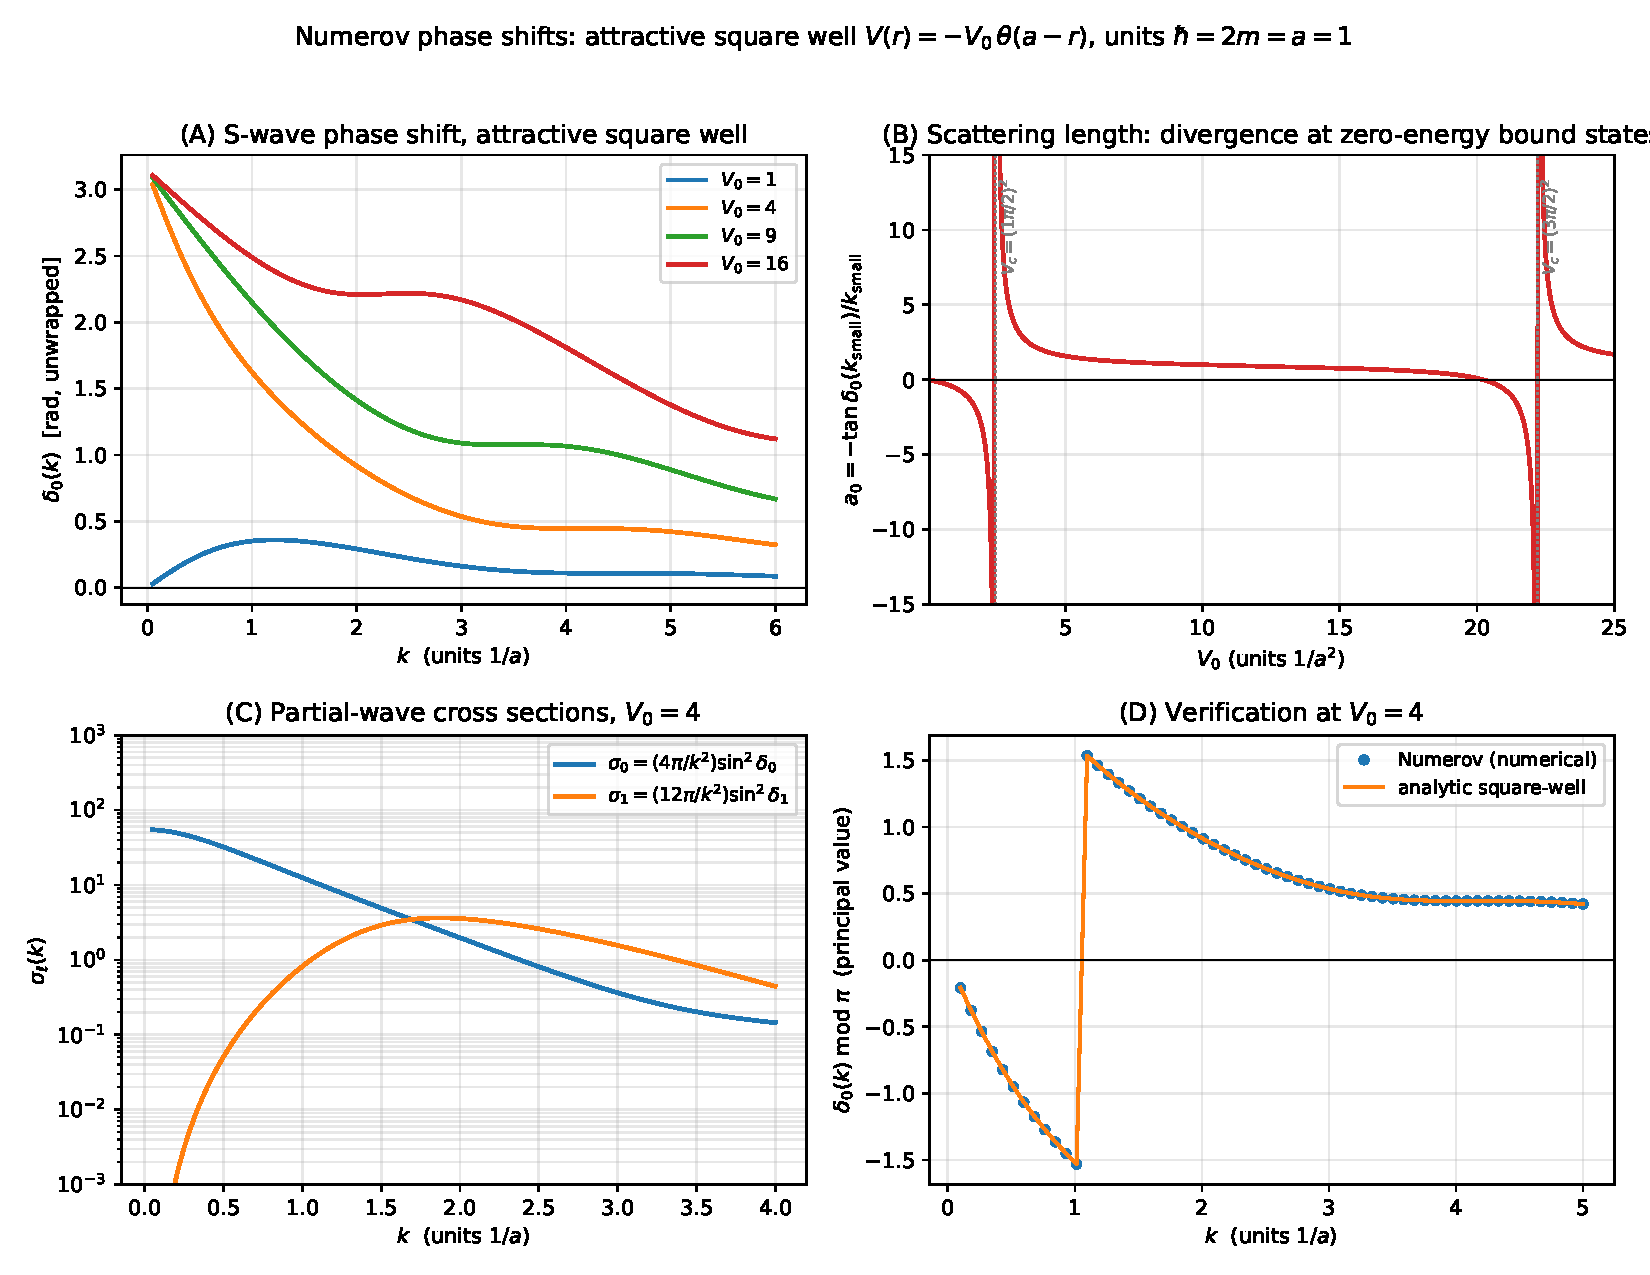
\includegraphics[width=0.95\linewidth]{ch10_numerov_phase}
    \caption{Numerov 法对吸引方势阱 $V(r)=-V_0\,\theta(a-r)$
    （单位 $\hbar=2m=a=1$）的 $s$、$p$ 波相移与截面。
    (A) $V_0=1,4,9,16$ 时的 $\delta_0(k)$（解 $\bmod\pi$ 后用
    \texttt{np.unwrap} 连续化）。$V_0=1<(\pi/2)^2\approx2.467$
    时无 $s$ 波束缚态，$\delta_0(0)=0$；$V_0=4,9,16$ 均处于
    $((\pi/2)^2,(3\pi/2)^2)$ 之间故各有 $1$ 个 $s$ 波束缚态，
    $\delta_0(0)\to\pi$，与 Levinson 定理 $\delta_0(0)=n_0\pi$
    （$n_0$ 为 $s$ 波束缚态数）一致。
    (B) 散射长度 $a_0=-\lim_{k\to0}\tan\delta_0(k)/k$ 作为 $V_0$
    的函数；图中两条灰虚线 $V_c=(\pi/2)^2,(3\pi/2)^2$ 处 $a_0$
    发散，对应零能束缚态新出现的阈值。
    (C) $V_0=4$ 时分波截面
    $\sigma_\ell(k)=(4\pi/k^2)(2\ell+1)\sin^2\delta_\ell(k)$
    （对数刻度）；低能区 $\sigma_0\propto a_0^2$ 占主导，
    $\sigma_1$ 由 $k^4$ 阈值压低。
    (D) $V_0=4$ 时 Numerov 数值（蓝点）与解析公式
    $\tan(ka+\delta_0)=(k/K)\tan(Ka)$，$K=\sqrt{k^2+V_0}$
    （橙线，主值分支）的逐点对比。}
    \label{fig:numexp-ch10}
\end{figure}

\subsection*{物理讨论}
\paragraph{Levinson 定理。}
图~\ref{fig:numexp-ch10}(A) 直接验证 $\delta_\ell(0)=n_\ell\pi$：
$V_0=1$ 时 $n_0=0$、$\delta_0(0)=0$；$V_0=4,9,16$ 三者落在同一
$s$ 波束缚态阈值区间 $((\pi/2)^2,(3\pi/2)^2)\approx(2.467,22.207)$
内，$n_0=1$、$\delta_0(0)=\pi$。每跨过一个阈值
$V_c=((2n+1)\pi/2)^2$，$\delta_0(0)$ 跳一个 $\pi$，与
\eqref{eq:pw-Levinson} 完全一致。

\paragraph{散射长度发散。}
图~\ref{fig:numexp-ch10}(B) 展示了 $a_0(V_0)$ 在
$V_c=(\pi/2)^2,(3\pi/2)^2$ 附近的极点，对应零能束缚态出现：
$a_0\to-\infty$（束缚态即将形成）→ 出现束缚态后 $a_0\to+\infty$
→ 回落至有限值。这是有效程展开
\[
  k\cot\delta_0(k)=-\frac{1}{a_0}+\frac12 r_0 k^2+\cdots
\]
中 $a_0$ 的奇异行为，物理上对应弱束缚极限下的“共振增强”——
低能截面 $\sigma_0\to 4\pi a_0^2$ 趋于无穷，正是冷原子物理中
Feshbach 共振、核物理中氘核虚态等现象的方势阱模型对应物。

\paragraph{低分波主导与解析比对。}
图~\ref{fig:numexp-ch10}(C) 展示低能区 $\sigma_0\gg\sigma_1$，
来源于离心位垒造成的 $\sigma_\ell\propto k^{4\ell}$ 阈值行为；
随 $k$ 增大高分波逐次开启，$ka\sim 1$ 起 $\sigma_1$ 与 $\sigma_0$
可比。图~\ref{fig:numexp-ch10}(D) 显示 Numerov 数值与方势阱
$s$ 波解析公式在主值分支上完全吻合（误差 $\lesssim 10^{-3}$，
与步长 $h=10^{-3}$ 的 $\mathcal O(h^4)$ 全局精度一致），
说明该数值方案可靠地推广到任意（球对称）势 $V(r)$。
